\documentclass[letterpaper, 12pt, oneside]{tesis}

\usepackage[spanish]{babel}
\selectlanguage{spanish}
\usepackage[utf8]{inputenc}
\usepackage[fixlanguage]{babelbib}
\usepackage[T1]{fontenc}
\usepackage{natbib}
\usepackage{enumerate}
\usepackage{tikz}
\usepackage{color}
\usepackage{verbatim}
\usepackage{fancyvrb}
\usepackage{hyperref}
\hypersetup{urlcolor=blue, colorlinks=false}
\usepackage{amsmath}
\usepackage{amsthm}
\usepackage{amssymb}
\usepackage{mdframed}
\usepackage{blindtext}
\usepackage{paralist}
\usepackage{parskip}
\usepackage[noend]{algpseudocode}
\usepackage[chapter]{algorithm}

\floatname{algorithm}{Algoritmo}
\renewcommand{\algorithmicrequire}{\textbf{Input:}}
\renewcommand{\algorithmicensure}{\textbf{Output:}}

\graphicspath{{img/}}

% Sangrías de 3 espacios (3 veces el espacio de la x)
\parindent 3ex 
% Interlineado
\setlength{\baselineskip}{1.5pt}
% Interpárrafo
%\setlength{\parskip}{16.5pt}

\topmargin 2cm

\renewcommand{\tablename}{Tabla}

\newcommand\listsymbolname{Acrónimos y Símbolos}

% Definiciones
\theoremstyle{definition}
\newtheorem{definicion}{Definición}

% Portada
\begin{titlepage}
    \title{\vspace{-2cm} 
\includegraphics[width=1.2in]{./usb.pdf} \\[.2cm]
        \large Universidad Simón Bolívar \\
        Decanato de Estudios Profesionales \\
        Coordinación de Ingeniería de la Computación
        \vfill \LARGE @títuloProyecto \vfill}
    \author{Por: \\
        Alejandro Flores V. \\[1.2cm]
        Realizado con la asesoría de: \\
        Emely Arraiz B.\\[1.2cm]
        PROYECTO DE GRADO \\
Presentado ante la Ilustre Universidad Simón Bolívar \\
como requisito parcial para optar al título de \\
Ingeniero de Computación}
    \date{Sartenejas, septiembre de 2014}
\end{titlepage}

\begin{document}
\frontmatter
\maketitle
\setstretch{1.3}


% +------+
% | ACTA |
% +------+
% Pagina del acta final
\begin{titlepage}
\begin{center}

% Upper part

\includegraphics[scale=0.5]{usb.pdf} \\

\textsc {\large UNIVERSIDAD SIMÓN BOLÍVAR} \\
\textsc{DECANATO DE ESTUDIOS PROFESIONALES\\
COORDINACIÓN DE INGENIERÍA DE LA COMPUTACIÓN}

\bigskip
\bigskip
\bigskip
\bigskip
\bigskip
\bigskip

% Title
\textsc{ACTA FINAL PROYECTO DE GRADO}

\bigskip
\bigskip

\textsc{\bfseries @títuloProyecto}

\bigskip
\bigskip
\bigskip
\bigskip

\begin{minipage}{\textwidth}
\centering
Presentado por: \\
\textsc{\bfseries Alejandro Flores V.} \\

\bigskip
\bigskip
\bigskip

Este Proyecto de Grado ha sido aprobado por el siguiente jurado examinador: \\

\bigskip
\bigskip

% Despues de cada line coloca el (los) nombre(s) de
% cada uno de los integrantes del jurado.
\line(1,0){200} \\
Emely Arráiz B.\\

\bigskip
\bigskip

\line(1,0){200} \\
@jurado1\\

\bigskip
\bigskip

\line(1,0){200} \\
@jurado2\\
\end{minipage}

\bigskip
\bigskip
\vfill

% Date/Fecha
{\large \bfseries Sartenejas, @día de @mes de @año}

\end{center}
\end{titlepage}


% +---------+
% | RESUMEN |
% +---------+
\addtotoc{Resumen}
\abstract{
\addtocontents{toc}{\vspace{1em}}

En este trabajo se considera el problema de \emph{Selección de Instancias} (SI), como estrategia de reducción de datos durante la aplicación de procesos de KDD.
Estando los datos agrupados en instancias independientes (una entrada en una base de datos), el problema de SI busca seleccionar el subconjunto de instancias de menor cardinalidad, que mantenga o mejore la precisión de clasificación al ser usado como conjunto de entrenamiento.
El estudio de este problema se ha popularizado a lo largo de los últimos años debido a la creciente necesidad de reducir los datos a ser almacenados y posteriormente analizados.
Dada su inherente complejidad, los trabajos sobre el problema de SI se han centrado en la formulación de algoritmos heurísticos que puedan generar (en tiempos aceptables) buenas soluciones al problema.
Durante la última década, numerosos autores han acudido al uso de metaheurísticas para encontrar soluciones al problema de SI, debido a su comprobada capacidad para encontar buenas soluciones a gran variedad de problemas.
En el presente trabajo se implementan 5 metaheurísticas (\emph{i.e.} GGA, SGA, CHC, PBIL y PSO) para conseguir soluciones al problema de SI. Adicionalmente, se proponen una serie de modificaciones sobre las estrategias de generación de soluciones iniciales, con la finalidad de reducir la cardinalidad de las soluciones encontradas y guiar el inicio de la búsqueda a soluciones que satisfagan los objetivos del problema. La evaluación experimental muestra que la disminución de la probabilidad de aparición de bits al $5\%$ permite una disminución sustancial de los tiempos de ejecución de las metaheurísticas, mejorando los resultados en términos de la reducción alcanzada, y sin afectar negativamente la precisión del clasificador. Adicionalmente, un estudio comparativo entre las metaheurísticas evaluadas, concluye que PBIL obtiene los mejores resultados en función de los objetivos del problema. Sin embargo, el comportamiento exhibido por CHC resulta interesante con miras en su aplicación a conjuntos de datos de mayor tamaño, puesto que es la metaheurística que se ve menos afectada por el número de instancias.

}

% Las palabras clave son generalmente los nombres de áreas de investigación a
% los cuales está asociado el trabajo. Generalmente son tres o cuatro.
\noindent \begin{small} \textbf{Palabras clave}: reducción de datos, selección de instancias, metaheurísticas.
\end{small}


\clearpage
\setstretch{1.3}

% +-----------------+
% | AGRADECIMIENTOS |
% +-----------------+
\acknowledgements{
\addtocontents{toc}{\vspace{1em}}

\blindtext

}
\clearpage


\pagestyle{fancy}

% +--------+
% | INDICE |
% +--------+
\lhead{\emph{Índice General}}
\tableofcontents

\lhead{\emph{Índice de Figuras}}
\listoffigures

\lhead{\emph{Índice de Tablas}}
\renewcommand*\listtablename{Índice de Tablas}
\listoftables

\lhead{\emph{Índice de Algoritmos}}
\renewcommand*\listalgorithmname{Índice de algoritmos}
\listofalgorithms
\addcontentsline{toc}{chapter}{Índice de algoritmos}

% +----------------------+
% | ACRONIMOS Y SIMBOLOS |
% +----------------------+
\setstretch{1.5}
\clearpage
\lhead{\emph{Acrónimos y símbolos}}
\listofsymbols{ll}
{

    % Aquí van las siglas
    \textbf{KDD} & Knowledge Discovery in Databases\\
    \textbf{MD}  & Minería de Datos\\
	\textbf{SI}  & Selección de Instancias\\
	\textbf{NN}  & Nearest Neighbor\\
%	\textbf{} & \\
%	\textbf{} & \\
    &\\
    \hline
    &\\

    % Aquí van los símbolos
    $\in$ & Relación de pertenencia, \guillemotleft\emph{es un elemento de}\guillemotright
}

\setstretch{1.3}


\pagestyle{empty}

% +--------------+
% | DECLARATORIA |
% +--------------+
\dedicatory{
    \textbf{Dedicatoria} \bigskip

    A @personasImportantes, por @razonesDedicatoria.
}

\addtocontents{toc}{\vspace{2em}}


\mainmatter
\pagestyle{fancy}

% +--------------+
% | INTRODUCCION |
% +--------------+

\chapter*{Introducción}
\label{intro}
\lhead{\emph{Introducción}}
\addcontentsline{toc}{chapter}{Introducción}

Durante las últimas décadas, los avances tecnológicos hay llevado a un aumento significativo en la cantidad de información generada por la actividad humana. Nuevos campos de estudio han emergido con la finalidad analizar esta enorme cantidad de datos. Bajo el contexto del campo de \emph{Descubrimiento de Conocimiento en Bases de Datos} (KDD por sus siglas en inglés), los procesos de \emph{Minería de Datos} (MD) buscan patrones en los conjuntos de datos con el objetivo de construir modelos de representación que permitan (entre otras cosas) clasificar datos desconocidos. Sin embargo, debido a que estos datos se encuentran agrupados en muestras de un evento particular (o instancias), surge el problema de aparición de instancias redundantes, con datos inconsistentes o ruidosos, etc. En este sentido, la reducción de los datos juega un rol fundamental en la aplicación efectiva de técnicas de MD.

El problema de \emph{Selección de Instancias} (SI) busca escoger un subconjunto de las instancias originales, con la finalidad de reducir la cantidad de datos almacenados sin perjudicar (o incluso mejorando) la capacidad de representación original. Puede verse como un \emph{problema de optimización combinatoria} en el que cada instancia puede pertenecer o no al subconjunto seleccionado; esto implica un espacio de posibles soluciones de tamaño $2^n$, siendo $n$ el número de instancias iniciales. Este problema ha sido estudiado ampliamente por númerosos autores, por lo que existe abundante literatura sobre algorítmos heurísticos para encontrar soluciones al problema de SI.

Debido a que las metaheurísticas son métodos de búsqueda estocástica de propósito general, han sido adaptadas en numerosas ocaciones para encontrar soluciones a problemas de optimización combinatoria. Las metaheurísticas proveen un esquema de búsqueda flexible, que permite recorrer el espacio de soluciones de diversos problemas. Aunque no garantizan optimalidad, en general, las metaheurísticas son capaces de encontrar buenas soluciones en espacios de búsqueda particularmente grandes. Por esta razón, durante los últimos años, muchos autores han estudiado el uso de metaheurísticas para encontrar soluciones al problema de SI.

En este sentido, algunos de los primeros trabajos se centran en adaptar metaheurísticas de trayectoria para conseguir soluciones al problema de SI. Los trabajos de \emph{Cerverón et al.} \cite{cerveron2001another} y \emph{Zhang et al.} \cite{zhang2002optimal} introducen modificaciones al algoritmo de \emph{Búsqueda Tabú}. No obstante, la mayoria de los estudios se han enfocado en adaptaciones de \emph{Algoritmos Evolutivos}. En la literatura se encuentran adaptaciones de \emph{Algoritmos de Estimación de Distribución} \cite{sierra2001prototype}, \emph{Algoritmo Genético Inteligente} \cite{ho2002design}, \emph{Algoritmo Memético Estacionario} \cite{garcia2008memetic}, etc. Destaca el trabajo de \emph{Cano et al.} \cite{cano2003using}, que realiza un estudio comparativo entre algoritmos heurísticos al problema de SI y adaptaciones de \emph{Algoritmo Genético Generacional} (GGA), \emph{Algoritmo Genético Estacionario} (SGA), \emph{CHC Adaptive Search Algorithm} (CHC) y \emph{Population-Based Incremental Learning} (PBIL).

Sin embargo, el principal obstáculo para la aplicación de metaheurísticas en el problema de SI, es que se requiere un alto número de iteraciones para encontrar soluciones que cumplan satisfactoriamente los objetivos del problema en términos de reducción de los datos y precisión de representación.

En el presente trabajo se realiza un estudio comparativo entre 5 metaheurísticas: GGA, SGA, CHC, PBIL y PSO. En función de los obstáculos planteados, se proponen una serie de modificaciones a las estrategias de generación de soluciones iniciales de estas metaheurísticas. La idea es iniciar el proceso de búsqueda en regiones del espacio de soluciones que mejoren los resultados en términos de los objetivos del problema. Esto con la finalidad de reducir el número de iteraciones necesarias para alcanzar buenas soluciones al problema y así permitir su aplicación sobre conjuntos de datos con gran número de instancias.

Este trabajo está estructurado como sigue. En el Capítulo 1 se describe en amplitud el problema de SI y los enfoques seguidos en la literatura para su solución. En el Capítulo 2 se describen de forma general las metaheurísticas usadas en este estudio, mientras que en el Capítulo 3 se presentan las modificaciones propuestas sobre las metaheurísticas para conseguir soluciones al problema de SI y resolver el obstáculo mencionado. En el Capítulo 4 se detalla el diseño experimental seguido y se presentan y analizan los resultados obtenidos. Finalmente, se presentan las conclusiones y recomendaciones finales del trabajo.


% +-----------+
% | CAPITULOS |
% +-----------+
\chapter{Selección de Instancias}
\label{capitulo1}
\lhead{Capítulo 1. \emph{Selección de Instancias}}

Este capítulo describe el problema de \emph{Selección de Instancias} (SI), como estrategia de reducción de datos para la aplicación de técnicas de \emph{Minería de Datos} (MD). El problema es definido formalmente, se describen sus principales características y se realiza un breve análisis del estado del arte.

\section{Reducción de Datos}

Como parte del proceso de \emph{Descubrimiento de Conocimiento en Bases de Datos} (Knowledge Discovery in Databases o \emph{KDD}), la fase de preprocesamiento de los datos juega un rol fundamental para la aplicación efectiva de técnicas de \emph{Minería de Datos} (\emph{MD}). Una de las estrategias de mayor uso durante la fase de preprocesamiento es la de \emph{reducción de datos}.

El problema de \emph{reducción de datos} consiste en decidir qué datos deben ser utilizados durante la aplicación de algoritmos de MD con el objetivo de construir modelos representativos de los datos originales. Dicha decisión debe basarse en la relevancia de los datos con respecto a los objetivos que se persiguen, o inclusive, por limitaciones técnicas. En términos prácticos, la importancia del problema de \emph{reducción de datos} radica en los siguientes factores:
\begin{inparaenum}[\itshape a\upshape)]
\item \textit{Tiempo y Espacio}: Mientras mayor sea el número de datos a utilizar, mayor será el espacio necesario para almacenarlos y el tiempo requerido para analizarlos. 
\item \textit{Sensibilidad al ruido}: Al aumentar el número de instancias en el conjunto de datos, también lo hace la probabilidad de aparición de datos atípicos, inconsistentes o redundantes. Su eliminación se vuelve necesaria para evitar un impacto negativo en los modelos de representación creados a partir de los datos.
\end{inparaenum}

En función de estos criterios, y basados en la definición de los datos, se han formulado diferentes estrategias para llevar a cabo la fase de reducción. En los procesos de KDD, un conjunto de datos está definido en función de un conjunto de clases $\Omega$ y un conjunto $T$ de $n$ observaciones de un evento, cada una con $m$ mediciones, donde:\\

\begin{definicion}
Una \textbf{instancia} $t_i$ (con $i = 1\dots n$) es una observación del evento; donde $t_i = (v_{i,1}, v_{i,2}, \dots, v_{i,m})$ es una tupla de $m$ valores/mediciones (un punto en un espacio $m$-dimensional). Adicionalmente, cada instancia $t_i$ pertenece a la \emph{clase} $\omega_{t_i} \in \Omega$.\\
\end{definicion}

\begin{definicion}
Un \textbf{atributo} $p_j$ (con $j = 1\dots m$) define el conjunto de mediciones \guillemotleft\emph{de un mismo tipo}\guillemotright\ para todas las observaciones, \emph{i.e.} $p_j = \left\{ v_{i,j} \mid i = 1\dots n \right\}$. Cada atributo puede presentarse en diferentes formatos: \emph{nominales}, \emph{discretos}, o \emph{continuos}.
\end{definicion}

En la literatura se han definido varias estrategias para realizar el proceso de \emph{reducción de datos}. Entre ellas las más relevantes son:

\begin{itemize}
\item \textbf{Selección de Instancias}
\cite{DBLP:journals/ai/BlumL97,Liu:2002:IIS:593433.593525}: Busca la reducción del conjunto de datos mediante la selección de un subconjunto de instancias, de forma tal que dicho subconjunto conserve las capacidades de representación del conjunto original.
\item \textbf{Selección de Atributos}
\cite{DBLP:journals/ai/BlumL97, Liu:1998:FEC:551943}: Esta técnica permite eliminar atributos del conjunto de datos original, que no contribuyen (o que influyen negativamente) a la construcción de un modelo representativo.
\item \textbf{Discretización de Atributos}
\cite{DBLP:conf/ijcai/FayyadI93, Liu:2002:DET:593435.593535}: Esta estrategia busca convertir atributos \emph{continuos} en \emph{discretos} (cuantificando el espacio de posibles valores), o disminuir el número de valores \emph{discretos} (combinando valores adyacentes).
\end{itemize}

Digamos que se tiene una base de datos de pacientes en un hospital, y se desea entrenar un clasificador para predecir la existencia de enfermedades cardíacas en nuevos pacientes. Por cada paciente se registra su nombre, sexo, edad, altura, si es fumador o no, cuántas horas de ejercicio hace por semana, si tiene historia de enfermedades cardíacas en su familia, etc. Un algoritmo de selección de atributos eliminaría el atributo del nombre del paciente, puesto que no contribuye en la predicción esperada, mientras que siguiendo alguna estrategia de discretización de atributos, el atributo de edad podría dividirse en intervalos de 15 o 20 años. Finalmente, un algoritmo de selección de instancias buscará eliminar de la base de datos a pacientes con información faltante, repetidos o con valores fuera de lo común.

Este estudio se centra en el problema de \emph{Selección de Instancias}. En las siguientes secciones, el problema será definido formalmente y se describirán sus principales características.

\section{Selección de Instancias}

Dado un conjunto inicial de instancias $T = \left\{ t_i \mid i = 1 \dots n \right\}$ y un conjunto de clases $\Omega$, donde cada instancia está formada por una tupla de valores $t_i = (v_{i,1}, v_{i,2}, \dots, v_{i,m})$ y pertenece a la clase $\omega_{t_i} \in \Omega$, el problema de \emph{Selección de Instancias} (SI) consiste en seleccionar un subconjunto $R \subseteq T$ que mantenga (o mejore) la capacidad de representación del conjunto original $T$.

Este problema puede ser formulado como un \emph{problema de optimización combinatoria}, donde se busca el $R^* \subseteq T$ de menor cardinalidad que mantenga (o mejore) la capacidad de representación del conjunto original. Cada instancia perteneciente a $T$, puede o no pertenecer a $R$, lo que significa que el problema de SI tiene un espacio de posibles soluciones igual a $2^n$.

En particular, la literatura se ha enfocado en la aplicación del problema de SI para su uso en clasificadores \cite{DBLP:journals/corr/GottliebK14,DBLP:conf/jcdcg/Toussaint02}. El subconjunto seleccionado se usa como conjunto de entrenamiento, en base al cuál el clasificador estima la clase $\hat{\omega}$ de instancias previamente desconocidas. En este sentido, el problema de optimización de SI busca conseguir un $R^* \subseteq T$ \emph{consistente} y de cardinalidad mínima, donde:\\

\begin{definicion}
Un conjunto $R$ es \textbf{consistente} con $T$, \emph{si y solo si} toda instancia $t \in T$ es clasificada correctamente (\emph{e.i.} $\hat{\omega}_t = \omega_t$) mediante el uso de un clasificador \emph{M} y las instancias en $R$ como conjunto de entrenamiento.
\end{definicion}

La complejidad del problema de selección de instancias ha sido estudiada por diferentes autores: \emph{Bien} y \emph{Tibshirani} \cite{2012arXiv1202.5933B} describen una reducción del problema de SI al problema de \emph{Conjunto de Cobertura}, cuya versión de optimización es NP-Dura. Más aún, \emph{Wilfong} \cite{Wilfong:1991:NNP:109648.109673} y  \emph{Zukhba} \cite{Zukhba:2010:NPP:1921730.1921735} muestran que el problema de SI es NP-Duro.

En general, la literatura relacionada con el problema de SI se ha enfocado en el uso de clasificadores $k$-NN \cite{Garcia:2012:PSN:2122272.2122582} por su simplicidad y sobretodo, por su capacidad de representación de modelos sin información adicional sobre la distribución de los datos. El caso particular del problema de SI usando clasificadores $k$-NN también es conocido como \emph{Selección de Prototipos}. A continuación se describen estos clasificadores.

\subsection{Regla del Vecino Más Cercano (NN)}

Inicialmente descrita por \emph{Fix} y \emph{Hodges} \cite{fix_51_discriminatory}, la regla del \emph{Vecino Más Cercano} (Nearest Neighbor o NN) es una regla de inferencia basada en la idea de que instancias con atributos similares (cercanas en un espacio de $m$ dimensiones) tienden a compartir la misma clase. La regla NN estima la clase $\hat{\omega}_x$ de un punto $x$ en un espacio $m$-dimensional, dado un conjunto $T$ de instancias de entrenamiento y una función de distancia $\varphi$ entre dos puntos en dicho espacio:

\begin{equation}
\hat{\omega}_x = \omega_{t^*}\ ,\ 
t^* = \operatorname*{arg\,min}_{t\ \in\ T} \varphi(t,x)
\end{equation}

La generalización de la regla de inferencia NN se conoce como el clasificador $k$-NN: dado un $k \in \mathbb{N}$, se estima la clase $\hat{\omega}_x$ de un punto $x$ en función a la clase de las $k$ instancias más cercanas a $x$. En general, se usa la estrategia del \guillemotleft\emph{voto de la mayoría}\guillemotright, asignando la clase más común entre las $k$ instancias más cercanas. En particular, el clasificador 1-NN corresponde a la regla NN.

$k$-NN es un clasificador no paramétrico de \emph{aprendizaje perezoso} (debido a que la etapa de aprendizaje consiste en guardar el conjunto de entrenamiento), caracterizado por su sencillez en términos de implementación. Esa simplicidad y su probada utilidad para numerosas aplicaciones, han hecho del clasificador $k$-NN uno de los más estudiados en la literatura.

Uno de los trabajos de mayor relevancia es el de \emph{Cover} y \emph{Hart} \cite{Cover:2006:NNP:2263261.2267456}, quienes mostraron que cuando el número de instancias de entrenamiento tiende a infinito, el clasificador $k$-NN garantiza un error no mayor al doble de la tasa de error de Bayes: la menor tasa de error posible para un clasificador dado. Adicionalmente, probaron que para un conjunto de entrenamiento de cardinalidad finita, el clasificador 1-NN es admisible dentro de la clase de clasificadores $k$-NN: \emph{e.i.} No existe $k > 1$ tal que $k$-NN tenga menor probabilidad de error frente a 1-NN, para toda posible distribución de los datos.

Adicionalmente, algunos trabajos en geometría computacional han contribuido significativamente en la comprensión del problema. En este sentido, el clasificador 1-NN para espacios euclidianos puede definirse de forma alternativa en función de \emph{Diagramas de Voronoi} \cite{voronoi1908nouvelles}: una partición del espacio $\mathbb{R}^m$ en \emph{Celdas de Voronoi}, cada una definida por una instancia $t \in T$ donde $t$ es el \emph{vecino más cercano} para todos los puntos dentro del espacio dentro de dicha celda (ver Figura \ref{voronoi}). Esto ha permitido el desarrollo de nuevos enfoques para la búsqueda de vecinos más cercanos basados en \emph{Diagramas de Voronoi}, como el descrito por \emph{Kolahdouzan} y \emph{Shahabi} \cite{Kolahdouzan:2004:VKN:1316689.1316762}.

\begin{figure}[h!]
\centering
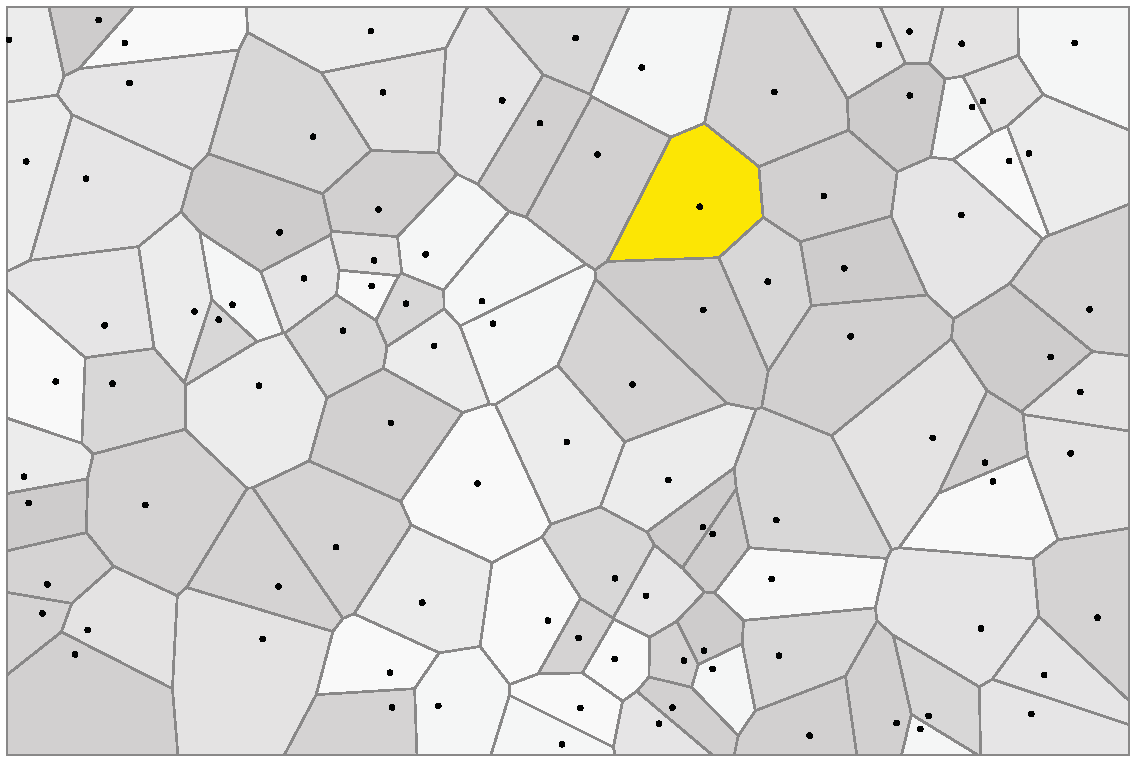
\includegraphics[width=0.6\textwidth]{voronoi.pdf}
\caption[Diagramas de Voronoi y NN]{Diagrama de Voronoi para instancias en un espacio $\mathbb{R}^2$. En amarillo la Celda de Voronoi de un punto $t \in T$, representando el espacio de puntos para los que $t$ es su \emph{vecino más cercano}.}
\label{voronoi}
\end{figure}

Similarmente, esta relación ha permitido avances importantes en términos de complejidad. En particular, mediante el uso de \emph{kd}-trees \cite{Bentley:1975:MBS:361002.361007} (árboles de búsqueda binaria en múltiples dimensiones) se ha logrado disminuir la complejidad en tiempo de clasificación, de $\mathcal{O}(n)$ (de un enfoque ``ingenuo'' revisando todas las instancias) a $\mathcal{O}(\log{n})$, a costas de un aumento en el tiempo necesario para el entrenamiento del clasificador: de $\mathcal{O}(1)$ a $\mathcal{O}(n\log{n})$, el tiempo necesario para la construcción del árbol.

Sin embargo, los clasificadores $k$-NN presentan ciertas propiedades desalentadoras; el problema de conseguir el vecino más cercano de un punto dado, requiere --en cualquiera de los casos-- almacenar todas las instancias de entrenamiento: \emph{e.i.} $\mathcal{O}(n)$ en espacio. Adicionalmente, trabajos más recientes \cite{DBLP:conf/soda/KrauthgamerL04} muestran que en espacios euclidianos de altas dimensiones, la búsqueda del vecino más cercano requiere $\mathcal{O}(n)$ en tiempo: un fenómeno conocido como la \guillemotleft\emph{maldición de la dimensionalidad}\guillemotright\ (\emph{curse of dimensionality} en inglés). Finalmente, según \emph{Shwartz} y \emph{David} \cite{shalev2014understanding} los clasificadores NN tienden a sobre-ajustar el modelo con respecto al conjunto de entrenamiento (\emph{overfitting} en inglés); efecto que puede mitigarse aumentando el $k$ del clasificador \cite{devroye1994strong, shalev2014understanding} y eliminando instancias del conjunto de datos \cite{DBLP:journals/corr/GottliebKK13}.

\paragraph*{Algunas definiciones}
A continuación se definen algunos conceptos relevantes para la descripción de métodos heurísticos de SI en futuras secciones. Para un subconjunto de instancias cualquiera $Q \subseteq T$:\\

\begin{definicion}
Los \textbf{asociados} en $Q$ de una instancia $t$ son aquellas instancias en $Q$ para las cuales $t$ pertenece a su conjunto de $k$ instancias más cercanas:
\begin{equation}
\emph{asociados}_Q(t) = \left\lbrace q \in Q \mid t\in \emph{kNN}(q) \right\rbrace
\end{equation}
\end{definicion}

\begin{definicion}
Los \textbf{enemigos} en $Q$ de una instancia $t \in T$ son aquellas instancias en $Q$ con una \emph{clase} diferente a la \emph{clase} de $t$:
\begin{equation}
\emph{enemigos}_Q(t) = \left\lbrace q \in Q \mid \omega_{q} \neq \omega_{t} \right\rbrace
\end{equation}
\end{definicion}

\begin{definicion}
El \textbf{enemigo más cercano} (\emph{nearest enemy} o NE) en $Q$ de una instancia $t \in T$, es la instancia más cercana a $t$ con diferente clase, y es denotada como $\mathrm{NE}_Q(t)$. \emph{i.e.} $\mathrm{NE}_Q(t)$ es la instancia más cercana a $t$ perteneciente a $\emph{enemigos}_Q(t)$:
\begin{equation}
\mathrm{NE}_Q(t) = \operatorname*{arg\,min}_{e\ \in\ \emph{enemigos}_Q(t)} \varphi(t,e)
\end{equation}
\end{definicion}

\section{Algoritmos de aproximación para Selección de Instancias}
\label{alg-aprox-si}

Debido a la complejidad del problema de SI, la literatura se ha enfocado en la definición de algoritmos heurísticos para conseguir soluciones aproximadas. De nuevo, el uso de clasificadores $k$-NN es una práctica extendida a lo largo de estos trabajos, por lo que las características de la regla NN han servido de inspiración para el desarrollo de la mayoría de los métodos de selección. Sin embargo, otras propuestas se basan en el orden de revisión de las instancias, así como en la realización de un muestreo aleatorio sobre el conjunto de datos. Finalmente, algunos enfoques se centran en aplicar procesos de búsqueda de propósito general, guiados por los objetivos del problema.

A continuación se describen brevemente algunos de los algoritmos heurísticos más recurrentes en la literatura relacionada al problema de SI.

\subsection{Métodos basados en la regla NN}

\begin{itemize}
\item \emph{Condensed Nearest Neighbor} (CNN) \cite{Hart:2006:CNN:2263267.2267647}\\
Inicialmente el conjunto $R$ se inicializa con una instancia cualquiera. Luego se itera sobre cada instancia $t \in T$; si $t$ no es clasificada correctamente usando $R$, $t$ se agrega a $R$.
CNN consigue un conjunto consistente, reduciendo considerablemente el conjunto de datos original. Sin embargo, no asegura un conjunto consistente mínimo, pues depende del orden en el que son revisadas las instancias en $T$.
\item \emph{Edited Nearest Neighbor} (ENN) \cite{wilson1972asymptotic}\\
Comienza con $R = T$. Luego itera sobre las instancias en $R$; aquellas que no sean bien clasificadas usando $R$ son eliminadas. Tiende a eliminar instancias ruidosas o cercanas a los bordes de decisión. Sin embargo, depende del orden en que itera sobre las instancias, y presenta bajas tasas de reducción dado que mantiene puntos internos.
\item \emph{Repeated Edited Nearest Neighbor} (RENN) \cite{wilson1972asymptotic}\\
Aplica ENN al conjunto de datos $R$ (inicialmente $R = T$) hasta que no ocurran cambios en $R$. Amplía la distancia entre clases y ``suaviza'' los bordes de decisión.
\item \emph{Reduced Nearest Neighbor} (RNN) \cite{DBLP:journals/tit/Gates72}\\
RNN extiende a CNN, usándola como solución inicial $R = R_{CNN}$. Luego, itera sobre cada instancia $t \in R$: si todas las instancias en $T$ son correctamente clasificadas usando $R\setminus\left\lbrace t \right\rbrace$, se elimina $t$ de $R$. En caso contrario, se mantiene $R$ y continua la iteración. La precisión de RNN puede mejorar respecto a CNN, pero es más costoso y su consistencia depende de la consistencia del conjunto resultante de CNN y del orden en que se iteren las instancias en $R$.
\end{itemize}

\subsection{Métodos basados en eliminación ordenada}

\begin{itemize}
\item \emph{Decremental Reduction Optimization Procedure 1} (DROP1) \cite{Wilson:1997:IPT:645526.657143}\\
Comienza con una solución inicial $R = T$. Itera sobre cada instancia $t \in R$: si todos sus \emph{asociados} en $R$ son correctamente clasificados con $R\setminus\left\lbrace t \right\rbrace$, $t$ se elimina de $R$. Reduce considerablemente el conjunto de datos inicial, pero obtiene baja precisión de clasificación, y el subconjunto resultante depende del orden en que se iteró sobre $T$.
\item \emph{Decremental Reduction Optimization Procedure 2} (DROP2) \cite{Wilson:1997:IPT:645526.657143}\\
Es una mejora sobre DROP1 en la cuál se elimina una instancia $t$ cuando todos sus \emph{asociados} en $T$ son clasificadas correctamente usando $R\setminus\left\lbrace t \right\rbrace$. Además, DROP2 ordena las instancias con respecto a la distancia de su \emph{enemigo} más cercano, en un intento de eliminar primero instancias centrales, y luego los puntos en los bordes de decisión.
\item \emph{Decremental Reduction Optimization Procedure 3} (DROP3) \cite{Wilson:1997:IPT:645526.657143}\\
Dado que el orden en que se iteran las instancias en DROP2 se ve alterado por puntos ruidosos, DROP3 filtra instancias ruidosas antes de ordenar el conjunto de entrenamiento.
\end{itemize}

\subsection{Métodos basados en muestreo aleatorio}

\begin{itemize}
\item \emph{Random Mutation Hill Climbing} (RMHC) \cite{DBLP:conf/icml/Skalak94}\\
Se selecciona un subconjunto de instancias aleatorias $R$ de tamaño fijo. En cada iteración el algoritmo intercambia una instancia en $R$ por una en $T \setminus R$; si el cambio mejora la precisión, se mantiene, en caso contrario se deshace.
\end{itemize}

\subsection{Métodos basados en metaheurísticas}

Las metaheurísticas son métodos de búsqueda estocástica de propósito general, usadas para encontrar soluciones óptimas o casi óptimas a problemas de optimización combinatoria. Por esta razón, muchos trabajos se han enfocado en el uso de estas técnicas para conseguir soluciones al problema de SI.

Algunos de los primeros trabajos se enfocaron en adaptar el algoritmo de \emph{Búsqueda Tabú} para solucionar el problema de SI. En particular, los estudios de \emph{Cerverón et al.} \cite{cerveron2001another} y \emph{Zhang et al.} \cite{zhang2002optimal} describen dos enfoques diferentes de modificación del algoritmo.

Sin embargo, la mayoría de los estudios se han enfocado en el uso de \emph{Algoritmos Evolutivos} (AE), adaptándolos para la búsqueda de soluciones al problema de selección. Entre ellos destaca el trabajo realizado por \emph{Cano et al.} \cite{cano2003using}; un completo estudio comparativo entre algoritmos ``tradicionales'' de SI y adaptaciones del \emph{Algoritmo Genético Generacional} (GGA), \emph{Algoritmo Genético Estacionario} (SGA), \emph{CHC Adaptive Search Algorithm} (CHC) y \emph{Population-Based Incremental Learning} (PBIL). Con este estudio, resulta evidente la utilidad de los \emph{AE} frente a los algoritmos tradicionales de SI en función de la capacidad de reducción y precisión de los conjuntos seleccionados.

Existen también otras adaptaciones y modificaciones sobre AE, entre los que destacan: \emph{Estimation of Distribution Algorithm} (EDA) \cite{sierra2001prototype}, \emph{Intelligent Genetic Algorithm} (IGA) \cite{ho2002design}, \emph{Steady-State Memetic Algorithm} (SSMA) \cite{garcia2008memetic} y \emph{Genetic Algorithm} \cite{gil2008evolving} basado en Error Cuadrático Medio, \emph{Clustered Crossover} y \emph{Fast Smart Mutation} (GA-MSE-CC-PSM).

%\subsection{Taxonomía}
%
%Debido a los numerosos enfoques existentes para aproximar soluciones al problema de SI, el trabajo de \emph{García} \emph{et al.} \cite{Garcia:2012:PSN:2122272.2122582} describe un esquema taxonómico para caracterizar las diferentes estrategias que se han desarrollado en base al uso de clasificadores $k$-NN. Dicho esquema clasifica las heurísticas de acuerdo al tipo de selección, y al tipo de evaluación y dirección de la búsqueda (ver Figura \ref{graphtaxonomia}).
%
%\begin{figure}[h!]
%\centering
%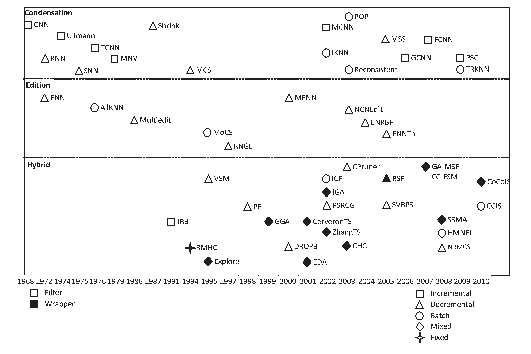
\includegraphics[width=0.7\textwidth]{taxonomia.pdf}
%\caption[Taxonomía de algoritmos de SI]{Taxonomía de algoritmos de aproximación\\para el problema de SI \cite{Garcia:2012:PSN:2122272.2122582}.}
%\label{graphtaxonomia}
%\end{figure}
%
%\noindent{\textbf{Según la dirección de la búsqueda}}\\
%La dirección en la cuál procede la búsqueda de posibles subconjuntos $R$ del conjunto inicial $T$ puede darse de diferentes formas.
%\begin{itemize}
%\item \emph{Incremental}:
%Comienzan con un conjunto $R$ vacio, o con unas pocas instancias representativas de cada clase en el conjunto de datos. En cada iteración se añaden nuevas instancias a $R$. Estos métodos tienden a ser más rápidos, pero dependen del orden de iteración sobre las instancias, y pueden producir un elevado \emph{overfitting}.
%\item \emph{Decremental}:
%Inicialmente $R = T$, y en cada iteración se eliminan elementos de $R$. Tienen la ventaja de contar inicialmente con todo el conjunto de datos para poder tomar decisiones, aunque son más costosos y dependen del orden de revisión de las instancias.
%\item \emph{Batch}:
%Estos métodos identifican aquellas instancias que cumplen cierto criterio, para luego eliminarlas/añadirlas todas como un conjunto. Presentan mayor complejidad.
%\item \emph{Mixed}:
%Comienzan con una selección aleatoria o con la selección dada por otro método de SI, para posteriormente añadir o eliminar instancias. Generalmente presentan \emph{overfitting}, además incrementar el tiempo de cómputo.
%\item \emph{Fixed}:
%Se refiere a una subcategoría de las heurísticas \emph{Mixed}, en la cuál se añaden y eliminan el mismo número de instancias; lo cuál no modifica el tamaño de la solución inicial.
%\end{itemize}
%
%\noindent{\textbf{Según el tipo de selección}}\\
%Varian en los tipos de instancias que seleccionan: puntos borde, centrales o cualesquiera.
%\begin{itemize}
%\item \emph{Condensation}:
%Seleccionan instancias cercanas a los bordes de decisión, también llamados puntos borde. Presentan mucha sencibilidad ante instancias ruidosas. En general estos métodos tienden a preservar la precisión para el conjunto de entrenamiento, pero afectan negativamente la generalización.
%\item \emph{Edition}:
%Buscan eliminar puntos borde para mantener bordes de decisión más ``suaves'', por lo que presentan menor sencibilidad ante puntos ruidosos. Tienden a mejorar la generalización del conjunto $T$ pero presentan un bajo porcentaje de reducción.
%\item \emph{Hybrid}:
%Permiten la selección de puntos borde y centrales con el objetivo de conseguir el menor conjunto $R$ que mantenga o aumente la precisión general del clasificador.
%\end{itemize}
%
%\noindent{\textbf{Según la evaluación de la búsqueda}}\\
%Diferentes estrategias para la evaluación de soluciones intermedias.
%\begin{itemize}
%\item \emph{Wrapper}:
%Utilizan el conjunto de datos completo sobre el clasificador\linebreak$k$-NN para la evaluación de soluciones intermedias, aplicando el esquema de validación \emph{leave-one-out}.
%\item \emph{Filter}:
%Usan solo partes del conjunto de datos original para la evaluación de soluciones intermedias, y sin aplicar el esquema de validación \emph{leave-one-out}. Implica menor tiempo evaluación, a costas de menor precisión.
%\end{itemize}

\subsection{Criterios de comparación}

Para comparar métodos de SI se consideran una serie de criterios usados para evaluar las ventajas y desventajas de cada algoritmo. A continuación se describen los factores más relevantes:

\begin{itemize}
\item \emph{Reducción}: El objetivo principal de métodos de SI es el de reducir el número de instancias del conjunto de datos. Esto no solo disminuye el espacio necesario para almacenar los datos, sino que acelera el proceso de clasificación.
\item \emph{Precisión}: Un algoritmo exitoso debe reducir el conjunto de datos, afectando en la menor medida posible su capacidad de generalización.
\item \emph{Tiempo}: A pesar de que el proceso de preprocesamiento y aprendizaje debe realizarse solo una vez, la complejidad de los algoritmos pueden volverlos poco prácticos para su uso sobre conjuntos de datos ``grandes''.
%\item \emph{Tolerancia al ruido}: Algoritmos que seleccionen consistentemente instancias atípicas o inconsistentes (``ruido'') presentan menor capacidad de generalización de los datos.
\end{itemize}

\chapter{Metaheurísticas para seleccionar instancias}
\label{capitulo2}
\lhead{Capítulo 2. \emph{Metaheurísticas para seleccionar instancias}}

\section{Metaheurísticas}

Las metaheurísticas son métodos estocásticos de búsqueda de propósito general sobre espacios combinatorios. Son usados generalmente para tratar problemas de optimización combinatoria, donde su complejidad hace imposible evaluar todas las soluciones factibles en un tiempo razonable; estos algoritmos son capaces de conseguir ``buenas'' soluciones a un problema en un período de tiempo mucho menor. Sin embargo, para muchos problemas la complejidad de estos algoritmos sigue siendo un factor prohíbitivo, debido al uso de funciones ``costosas'' para la evaluación de soluciones intermedias (\emph{fitness}).

La idea es desarrollar algoritmos que recorran solo una fracción del espacio de soluciones, y que sean capaces de encontrar soluciones óptimas o casi óptimas al problema en cuestión. Para lograrlo, las metaheurísticas combinan procesos de \emph{diversificación} e \emph{intensificación} (o \emph{exploración} y \emph{explotación} respectivamente) \cite{Yang:2008:NMA:1628847}. La fase de \emph{diversificación} implica la generación de soluciones diversas con el objeto de explorar el espacio de búsqueda, mientras que la fase de \emph{intensificación} se refiere al mejoramiento de soluciones (conseguir óptimos locales) mediante el uso de métodos de búsqueda local. La selección de las mejores soluciones asegura la convergencia a soluciones óptimas, mientras que la exploración aleatoria de soluciones evita que el algoritmo quede ``atrapado'' en óptimos locales. La combinación en el uso de ambos procesos hace posible conseguir buenas soluciones al problema sin la necesidad de recorrer el espacio de búsqueda completo.

Cada metaheurística está caracterizada por las estratégias que usa para cada fase, así como el orden y la frecuencia en que las aplica; esto permite clasificarlas en función de su similitud. En este sentido, a continuación se describe un conjunto de metaheurísticas caracterizadas por tener a la naturaleza como fuente de inspiración.

\section{Metaheurísticas inspiradas en la naturaleza}

La habilidad de la naturaleza para moldear soluciones a situaciones complejas, mediante procesos y reglas caracterizadas por su simplicidad, la ha convertido en una fuente inagorable de inspiración para el desarrollo de algoritmos de optimización. Estos algoritmos a menudo presentan buen desempeño para aproximar soluciones a todo tipo de problemas, dado que no requieren información sobre la distrubución del espacio de búsqueda. Por esta razón, existe una amplia literatura sobre enfoques bio-inspirados \cite{binitha2012survey} para resolver gran variedad de problemas en diversas áreas de computación.

En particular, los enfoques más comunes en la literatura sobre metaheurísticas inspiradas en la naturaleza se apoyan en
\begin{inparaenum}[\itshape a\upshape)]
\item la evolución de poblaciones (Algoritmos Evolutivos) y
\item el comportamiento colectivo (Inteligencia de Enjambre).
\end{inparaenum}

\subsection{Algoritmos Evolutivos}

Los Algoritmos Evolutivos (\emph{AE}) son metaheurísticas basadas en procesos de evolución biológica con el objetivo de explorar en amplitud espacios de solución con distribución desconocida. Con el fin de replicar los procesos evolutivos, los \emph{AE} mantienen un conjunto de soluciones candidatas al problema (una \emph{población} de \emph{cromosomas}/\emph{individuos}), que modifican iterativamente apoyandose en el uso de operadores de \emph{mutación}, \emph{recombinación} y/o \emph{selección}.

Los \emph{AE} codifican cada cromosoma como una cadena de genes (análogo a la estructura del ADN), donde cada gen representa una parte de la solución al problema en cuestión. A partir de esta representación, los \emph{AE} definen un conjunto de operadores que cumplen la función de las estrategias de \emph{exploración} y \emph{explotación}:

\begin{itemize}
\item \emph{Mutación}: Modifica los genes de soluciones intermedias con la finalidad de explorar el espacio de soluciones e introducir nueva información a la población. Simula la variabilidad en las poblaciones, fenómeno clave para la aparición de nuevos genes que aumenten la posibilidad de supervivencia.
\item \emph{Recombinación}/\emph{Crossover}: Permite el intercambio de información entre individuos de la población. Simula la reproducción entre individuos, necesaria para la transmisión de genes relevantes a las siguientes generaciones.
\item \emph{Selección}: Las estrategias de selección permiten definir aquellos individuos que participarán en la fase de reproducción, y por ende los genes que pasarán a la siguiente generación. Esto simula el proceso de selección natural en el que sobreviven los individuos mejor adaptados al ambiente.
\end{itemize}

En la literatura se han desarrollado diferentes esquemas que definen el uso de estos operadores. Los \emph{AE} más ``tradicionales'' son conocidos como \emph{Algoritmos Genéticos} (\emph{AG}) \cite{holland1975adaptation}, que suponen la aplicación más directa de los conceptos del proceso evolutivo. Sin embargo, dentro de la clase de \emph{AE} existe otro grupo de algoritmos que aplican dichos conceptos de forma diferente; la clase de \emph{Algorítmos de Estimación de Distribución} (``\emph{Estimation of Distribution Algorithm}'' - EDA) aplican los operadores de \emph{mutación}, \emph{recombinación} y \emph{selección} sobre una población de soluciones implicita en un modelo de distribución probabilístico.

A continuación se describen cuatro algoritmos pertenecientes a la clase de \emph{AE}: GGA, SGA y CHC, variantes del grupo de \emph{AG}, y PBIL, perteneciente a los \emph{EDA}.

\subsubsection{Generational Genetic Algorithm (GGA)}

GGA es el esquema ``tradicional'' de aplicación de los \emph{AG} \cite{back1996evolutionary,Muhlenbein91evolutionin}. Mantiene una población de individuos que evolucionan durante un número de iteraciones. Su principal característica es que en cada iteración se genera una nueva población, \emph{i.e.} un proceso de evolución \emph{generacional}.

En cada iteración el proceso evolutivo consiste en la creación de una nueva población de tamaño $\texttt{pop}$ mediante:
\begin{inparaenum}[\itshape a\upshape)]
\item la selección de los individuos para el proceso de reproducción (\emph{padres}),
\item la recombinación (con probabilidad $\texttt{cp}$) de pares de individuos \emph{padres} usando una estrategia particular de cruce/\emph{crossover}, y
\item la mutación de los individuos de la nueva población (llamados \emph{descendencia}), usando una probabilidad de mutación de cada gen igual a $\texttt{mp}$.
\end{inparaenum}
Ver el algoritmo \ref{gga-alg}.

\begin{algorithm}
\caption{Generational Genetic Algorithm}
\label{gga-alg}
\begin{algorithmic}[1]

\Require{\texttt{pop} tamaño de la población,
	\texttt{cp} probabilidad de cruce,
	\texttt{mp} probabilidad de mutación}
\Ensure{Una solución al problema}

\State $P \gets$ Generar población aleatoria de $\texttt{pop}$ individuos
\State $p^{*} \gets $ el \emph{mejor} individuo en $P$
\While{$\neg$ Condición de parada}
	\State $P' \gets \emptyset$
	\While{$\mid P' \mid < \texttt{pop}$}
		\State $p_1 \gets$ Seleccionar un individuo en $P$
		\State $p_2 \gets$ Seleccionar un individuo en $P$
		\State $c_1, c_2 \gets $ recombinar $p_1$ y $p_2$ con probabilidad $\texttt{cp}$
		\State Mutar $c_1$ y $c_2$ con probabilidad $\texttt{mp}$
		\State $P' \gets P' \cup \left\lbrace c_1, c_2 \right\rbrace$
	\EndWhile
	\State $P \gets P'$
	\If{El \emph{mejor} individuo en $P$ es \emph{mejor} que $p^{*}$}
		\State $p^{*} \gets$ el \emph{mejor} individuo en $P$
	\EndIf
\EndWhile
\State \Return $p^{*}$

\end{algorithmic}
\end{algorithm}

\subsubsection{Steady-State Genetic Algorithm (SGA)}

Descrito por \emph{Whitley et al.} \cite{whitley1988genitor}, SGA es una modificación del esquema general de \emph{AG} que sigue una estrategia reproductiva no generacional. SGA comienza con una población de tamaño $\texttt{pop}$, y en cada iteración se producen un máximo de dos nuevos individuos (no una nueva población).

En cada iteración
\begin{inparaenum}[\itshape a\upshape)]
\item se seleccionan dos individuos padres de la población actual,
\item se crea su descendencia (con probabilidad $\texttt{cp}$) mediante algún metodo de cruce/recombinación,
\item se agrega variabilidad mediante la mutación (con probabilidad $\texttt{mp}$) de la nueva descendencia, y
\item se sigue alguna estrategia de selección para reemplazar individuos en la población por la nueva descendencia, y así mantener el tamaño de la población igual a $\texttt{pop}$.
\end{inparaenum}
Ver el algoritmo \ref{sga-alg}.

\begin{algorithm}
\caption{Steady-State Genetic Algorithm}
\label{sga-alg}
\begin{algorithmic}[1]

\Require{\texttt{pop} tamaño de la población,
	\texttt{cp} probabilidad de cruce,
	\texttt{mp} probabilidad de mutación}
\Ensure{Una solución al problema}

\State $P \gets$ Generar población aleatoria de $\texttt{pop}$ individuos
\State $p^{*} \gets $ el \emph{mejor} individuo en $P$
\While{$\neg$ Condición de parada}
	\State $p_1 \gets$ Seleccionar un individuo en $P$
	\State $p_2 \gets$ Seleccionar un individuo en $P$
	\State $c_1, c_2 \gets $ recombinar $p_1$ y $p_2$ con probabilidad $\texttt{cp}$
	\State Mutar $c_1$ y $c_2$ con probabilidad $\texttt{mp}$
	\State Seguir algún criterio de reemplazo de individuos en $P$ por $c_1$ y $c_2$
	\If{El \emph{mejor} individuo en $P$ es \emph{mejor} que $p^{*}$}
		\State $p^{*} \gets$ el \emph{mejor} individuo en $P$
	\EndIf
\EndWhile
\State \Return $p^{*}$

\end{algorithmic}
\end{algorithm}

\subsubsection{CHC Adaptive Search Algorithm}

CHC se basa en el esquema de evolución generacional aplicado por GGA; mantiene una población de individuos de tamaño fijo ($\texttt{pop}$), generando una nueva población en cada iteración. Sin embargo, en cada iteración CHC aplica una estrategia de reemplazo ``elitista'', donde sobreviven los mejores $\texttt{pop}$ individuos entre la población actual y la descendencia producida.

La fase de reproducción aplicada por CHC tiene dos particularidades. En primer lugar, implementa un operador de recombinación llamado HUX, que intercambia la mitad de los genes que difieren entre los dos padres de forma aleatoria. Adicionalmente, CHC emplea ``prevención de incesto'': antes de realizar el cruce usando HUX, calcula la \emph{distancia de Hamming} entre ambos padres; si dicha distancia es mayor a cierto umbral (inicialmente $l/4$, donde $l$ es la longitud de los cromosomas), se realiza el cruce. En caso de no generarse ninguna descendencia durante una iteración particular, se disminuye el umbral en 1.

Durante el proceso de evolución de CHC no se aplica el operador de mutación: cuando el umbral de prevención de incesto llega a cero se considera que la población convergió, y comienza un proceso de repoblación en el que se usa la mejor solución encontrada hasta el momento. Se modifican hasta $35\%$ de sus genes de forma aleatoria para generar los $\texttt{pop}-1$ individuos restantes de la nueva población, y luego continuar el proceso evolutivo.

A continuación se presenta el pseudocódigo para CHC (algoritmo \ref{chc-alg}).

\begin{algorithm}
\caption{CHC Adaptive Search Algorithm}
\label{chc-alg}
\begin{algorithmic}[1]

\Require \texttt{pop} tamaño de la población
\Ensure Una solución al problema

\State $P \gets$ Generar población aleatoria de $\texttt{pop}$ individuos
\State $p^{*} \gets $ el \emph{mejor} individuo en $P$
\State $\mu \gets l/4$ \Comment Umbral de cruce
\While {$\neg$ Condición de parada}
	\For {$i \in [1 \dots \texttt{pop}/2]$}
		\State $p_1 \gets$ Seleccionar un individuo en $P$
		\State $p_2 \gets$ Seleccionar un individuo en $P$
		\If {$hamming(p_1,p_2) > \mu$}
			\State $c_1, c_2 \gets $ recombinar $p_1$ y $p_2$ usando HUX
			\State $P \gets P \cup \left\lbrace c_1, c_2 \right\rbrace$
		\EndIf
	\EndFor
	\If {$\mid P \mid = \texttt{pop}$}
		\State $\mu \gets \mu-1$
		\If {$\mu = 0$}
			\State $P \gets$ Generar población de $\texttt{pop}$ individuos usando $p^*$
			\State $\mu \gets l/4$
		\EndIf
	\Else
		\State $P \gets \texttt{pop}$ mejores individuos en $P$
		\If {El \emph{mejor} individuo en $P$ es \emph{mejor} que $p^{*}$}
			\State $p^{*} \gets$ el \emph{mejor} individuo en $P$
		\EndIf
	\EndIf
\EndWhile
\State \Return $p^{*}$

\end{algorithmic}
\end{algorithm}

\subsubsection{Population-Based Incremental Learning (PBIL)}

Esta metaheurística consiste en mantener un vector de probabilidades $V_p$ de tamaño $L$ (número de instancias iniciales), donde $V_p\left[i\right]$ es la probabilidad de que la $i$-esima instancia pertenezca a la solución ($i$-esimo bit sea 1).\\
Inicialmente $V_p\left[i\right] = 0.5\ \ \forall{i \in [1\dots L]}$. En cada iteración se sigue el siguiente proceso:

\begin{enumerate}[a)]
\item Se generan $N$ cromosomas (secuencias de bits) basados en las probabilidades en $V_p$.
\item Se acerca $V_p$ hacia la mejor solución generada $S_{best}$
$$V_p\left[i\right]=V_p\left[i\right]*(1-LR)+S_{best}\left[i\right]*LR$$
Donde $LR$ es la tasa de aprendizaje (\emph{learning rate}).
\item Se aleja $V_p$ de la peor solución generada $S_{worst}$\\
\noindent{Si $S_{best}\left[i\right] <> S_{worst}\left[i\right]$}
$$V_p\left[i\right]=V_p\left[i\right]*(1-Negat\_LR)+S_{best}\left[i\right]*Negat\_LR$$
Donde $Negat\_LR$ es la tasa de aprendizaje negativa.
\end{enumerate}

\begin{algorithm}
\caption{Population-Based Incremental Learning}
\label{pbil-alg}
\begin{algorithmic}[1]

\Require \texttt{pop} tamaño de la población,
	\texttt{mp} probabilidad de mutación,
	\texttt{ms} mutation shift,
	\texttt{lr} learning rate,
	\texttt{nlr} negative learning rate
\Ensure Una solución al problema

\State $V \gets$ Vector de probabilidades de tamaño $l$
\State $p^* \gets$ Una solución cualquiera
\While {$\neg$ Condición de parada}
	\State $P \gets$ Generar población de tamaño $\texttt{pop}$ según las probabilidades en $V$
	\State $b \gets $ El \emph{mejor} individuo en $P$
	\State $w \gets $ El \emph{peor} individuo en $P$
	\If {$b$ es \emph{mejor} que $p^{*}$}
		\State $p^{*} \gets b$
	\EndIf
	\For {$i \in [1 \dots l]$} \Comment{Actualizar el vector de probabilidades}
		\State $V_i \gets V_i * (1 - \texttt{lr}) + b_i * \texttt{lr}$
		\If {$b_i \neq w_i$}
			\State $V_i \gets V_i * (1 - \texttt{nlr}) + b_i * \texttt{nlr}$
		\EndIf
		\If {$\mathrm{Unif}(0,1) < \texttt{mp}$} \Comment{Mutación con probabilidad $\texttt{mp}$}
			\State $V_i \gets V_i * (1 - \texttt{ms}) + \mathrm{UnifDiscreta}(0,1) * \texttt{ms}$
		\EndIf
	\EndFor
\EndWhile
\State \Return $p^{*}$

\end{algorithmic}
\end{algorithm}

\subsection{Inteligencia de Enjambre}

\subsubsection{Particle Swarm Optimization (PSO)}

\emph{PSO} se inspira en el comportamiento de organismos biológicos, en particular, del vuelo de una bandada de aves. Cada ave o ``partícula'' (que representa una posible solución del espacio de búsqueda) tiene una velocidad asociada, y modifica su vuelo en relación a su propia experiencia, y a la experiencia de sus ``compañeras''. Diferentes estudios muestran que \emph{PSO} obtiene mejores resultados que los algoritmos genéticos (\emph{GA}), y en menor tiempo de cómputo.

Inicialmente se obtienen $P$ soluciones aleatorias, o partículas. Cada partícula $i$ está representada por un posición en un espacio $s$-dimensional \linebreak $\textbf{x}_i =\ <x_{i1},x_{i2},\dots,x_{is}>$. Luego, se realizan un número de iteraciones (\texttt{MAX\_ITER}) en las que se actualiza la posición de cada partícula de acuerdo a su velocidad $v_i$:

$$\textbf{x}_i = \textbf{x}_i + v_i$$

$$v_i = w v_i + c_1 Rand() (p_i - \textbf{x}_i) +  c_2 Rand() (p_g - \textbf{x}_i)$$

Donde $c_1$ y $c_2$ con constantes, $Rand()$ es una función aleatoria $[0,1]$, $p_i$ es la mejor solución encontrada por la partícula $i$ (de acuerdo a una función de evaluación/\emph{fitness} establecida), $p_g$ es la mejor solución global, y $w$ es el ``peso de inercia'' que establece la posible variabilidad de $v_i$. $w$ disminuye cada iteración de acuerdo a la siguiente fórmula:

$$w = \frac{(w_{start} - w_{end})(\texttt{MAX\_ITER} - \texttt{Iter})}{\texttt{MAX\_ITER} + w_{end}}$$

Siendo \texttt{Iter} la iteración actual del algoritmo, y $w_{start}$ y $w_{end}$ valores predeterminados.

\section{Adaptación para el problema de Selección de Instancias}

\subsection{Representación}

\subsection{Función objetivo}

\chapter{Adaptación al problema de Selección de Instancias}
\label{capitulo3}
\lhead{Capítulo 3. \emph{Adaptación al problema de Selección de Instancias}}

Al tratarse de métodos de búsqueda de propósito general, las metaheurísticas pueden modificarse para encontrar soluciones a todo tipo de problemas de optimización combinatoria. Para ello debe definirse la representación a usar, que permita codificar las posibles soluciones al problema, y una función de \emph{fitness} para evaluar dichas soluciones en función a los objetivos de optimización del problema.

A continuación se describen éstas y otras consideraciones generales para la aplicación de metaheurísticas al problema de \emph{Selección de Instancias}. Adicionalmente se plantea para cada metaheurística, las estrategias a usar durante el proceso de búsqueda, así como algunas modificaciones particulares.

\section{Consideraciones generales}

\subsection{Representación}

Una solución cualquiera al problema de \emph{SI} está dada por un subconjunto de instancias $R$ del conjunto inicial $T$ (\emph{i.e.} $R \subseteq T$). Por lo tanto, para un orden dado de las instancias $t_i \in T\ (i = 1 \dots n$, con $n = \vert T \vert)$, una codificación usando mapas de bits es suficiente para representar el espacio de soluciones al problema.

En este sentido, una solución particular al problema de \emph{SI} está descrita por un cromosoma $s$ de tamaño $n$, donde cada gen $s_i$ ($i = 1 \dots n$) es un \emph{bit} con valor 1/0 (``prendido'' o ``apagado'' respectivamente) que denota la pertenencia o no de la instancia correspondiente $t_i \in T$ al subconjunto seleccionado. $R_s \subseteq T$ es el subconjunto seleccionado representado por el cromosoma $s$, donde:

\begin{equation}
R_s = \left\lbrace t_i \in T \mid i = 1 \dots n \land s_i = 1 \right\rbrace
\end{equation}

Este conjunto $R_s$ permite evaluar la ``bondad'' de la solución $s$ en función de los objetivos de optimización del problema.

\subsection{Función de evaluación}

El objeto de la aplicación de metaheurísticas es conseguir soluciones óptimas o casi óptimas a gran variedad de problemas. Para ello es necesario definir una estrategia de comparación entre soluciones, \emph{i.e.} saber cuándo una solución es \guillemotleft\emph{mejor}\guillemotright\ que otra, que permita seleccionar aquellas soluciones que mejor se adapten a los objetivos del problema en cuestión.

Para el caso del problema de \emph{SI}, el objetivo es encontrar un subconjunto $R$ del menor tamaño posible, que mantenga un alto porcentaje de precisión de clasificación. \emph{Cano et. al} \cite{cano2003using} definen una función de evaluación que combina ambos objetivos en función de un parámetro $\alpha \in [0,1]$; a continuación se presenta una modificación de dicha función (su complemento), usada en el presente trabajo:

\begin{equation}
\mathit{fitness}(R) = \alpha\ \mathit{error}(R) + (1 - \alpha) \vert R \vert
\end{equation}

Donde $\mathit{error}(R)$ es el número de instancias en $T$ que son erróneamente clasificadas usando el conjunto $R \subseteq T$ como conjunto de entrenamiento de un clasificador 1-NN. El parámetro $\alpha$ combina los objetivos de la búsqueda: se usa $\alpha = 0.5$ siguiendo lo descrito por \cite{cano2003using} para obtener soluciones que satisfagan ambos objetivos del problema.

Para esta definción, el objetivo de las metaheurísticas para selección de instancias es \emph{minimizar} la función de evaluación descrita. Para ello deben minimizar ambos objetivos de la función; el error de clasificación usando el subconjunto seleccionado, y el tamaño de dicho subconjunto. En este sentido, dadas dos posibles soluciones $a$ y $b$, $a$ es \guillemotleft\emph{mejor}\guillemotright\ que $b$ si y solo si $\mathit{fitness}(R_a) < \mathit{fitness}(R_b)$.

\subsection{Generación de soluciones iniciales}
\label{generacion-sol-inic}

Para muchos problemas con esquemas de representación binaria, la generación de soluciones iniciales usada por metaheurísticas sigue una estrategia común: al generar un cromosoma aleatorio, cada bit tiene $50\%$ de probabilidad de estar prendido ($\delta = 0.5$). Esta estrategia genera soluciones con valor esperado de la mitad de los bits prendidos. Para el problema de \emph{SI} esto implica soluciones con una reducción inicial del $50\%$ sobre el conjunto $T$, y hace necesario un alto número de iteraciones para lograr obtener soluciones con reducciones significativas \cite{cano2003using}. Por esta razón, en el presente trabajo se usa una probabilidad de aparición del $5\%$ por cada bit ($\delta = 0.05$), generando soluciones iniciales con reducciones cercanas al $95\%$; el rol de la función objetivo no recae en disminuir los porcentajes de reducción de las soluciones, sino en mantenerlos en niveles aceptables, permitiendo explotar el espacio de búsqueda para conseguir soluciones con mayor precisión.

Sin embargo, el punto inicial de la búsqueda en términos de precisión sigue siendo aleatorio. Una estrategia común en metaheurísticas de trayectoria es la generación de soluciones iniciales usando algoritmos de aproximación; \emph{Cerveron et. al} \cite{cerveron2001another} plantean una modificación del algoritmo de Búsqueda Tabú para el problema de \emph{SI}, en la cuál usan CNN para generar la solución inicial de la búsqueda. Esta idea puede trasladarse a metaheurísticas poblacionales siguiendo un enfoque probabilístico: dada una selección inicial $R_0 \subseteq T$, los bits correspondientes a instancias en $R_0$ tienen mayor probabilidad de aparición que los bits de instancias en $T \setminus R_0$. Estas probabilidades constituyen un vector de probabilidades a ser usado por PBIL como vector inicial, o por los algoritmos genéticos (GGA, SGA y CHC) para generar soluciones iniciales. El algoritmo \ref{inicial-sol-alg} implementa este esquema de generación; para un $\delta$ particular (que determina el número de bits prendidos en las soluciones iniciales), el vector de probabilidades $V$ generado por el algoritmo cumple con que un máximo del $70\%$ de los bits prendidos en soluciones generadas usando $V$, pertenecen a la solución inicial $R_0$. Esto contribuye a guiar la búsqueda realizada por las metaheurísticas poblacionales, mientras se mantiene la variabilidad.

\begin{algorithm}
\caption{Generador de vector de probabilidades inicial}
\label{inicial-sol-alg}
\begin{algorithmic}[1]

\Require $R_0$ solución inicial
\Ensure Vector de probabilidades en base a $R_0$

\State{$hi \gets min(0.9, \frac{\delta \vert T \vert 0.7}{\vert R_0 \vert})$}
\State{$low \gets \frac{\delta \vert T \vert - hi \vert R_0 \vert}{\vert T \setminus R_0 \vert}$}
\State{$V \gets$ Vector de probabilidades de tamaño n}
\For{$i \in [1 \dots n]$}
	\If{$t_i \in R_0$}
		\State{$V_i \gets hi$}
	\Else
		\State{$V_i \gets low$}
	\EndIf
\EndFor
\State \Return{$V$}
\end{algorithmic}
\end{algorithm}

Cualquier solución generada por algoritmos de aproximación para el problema de \emph{SI} (sección \ref{alg-aprox-si}) sirve como ``semilla'' de este generador; en el presente trabajo se prueba el impacto del uso de soluciones iniciales calculadas por CNN. También se incluyen dos selecciones basadas en el órden según el \emph{enemigo más cercano} (NE - ``\emph{Nearest Enemy}''), seleccionando las instancias con mayor distancia NE (selección por \emph{Farthest NE}), o menor distancia NE (selección por \emph{Closest NE}). Finalmente, se prueba un método de selección propio llamado \emph{Nearest Enemy Hypersphere Selection} (NEHS). En la figura \ref{seleccion} se pueden observar los subconjuntos seleccionados por estas cuatro (4) estrategias.

\begin{figure}[h!]
\centering
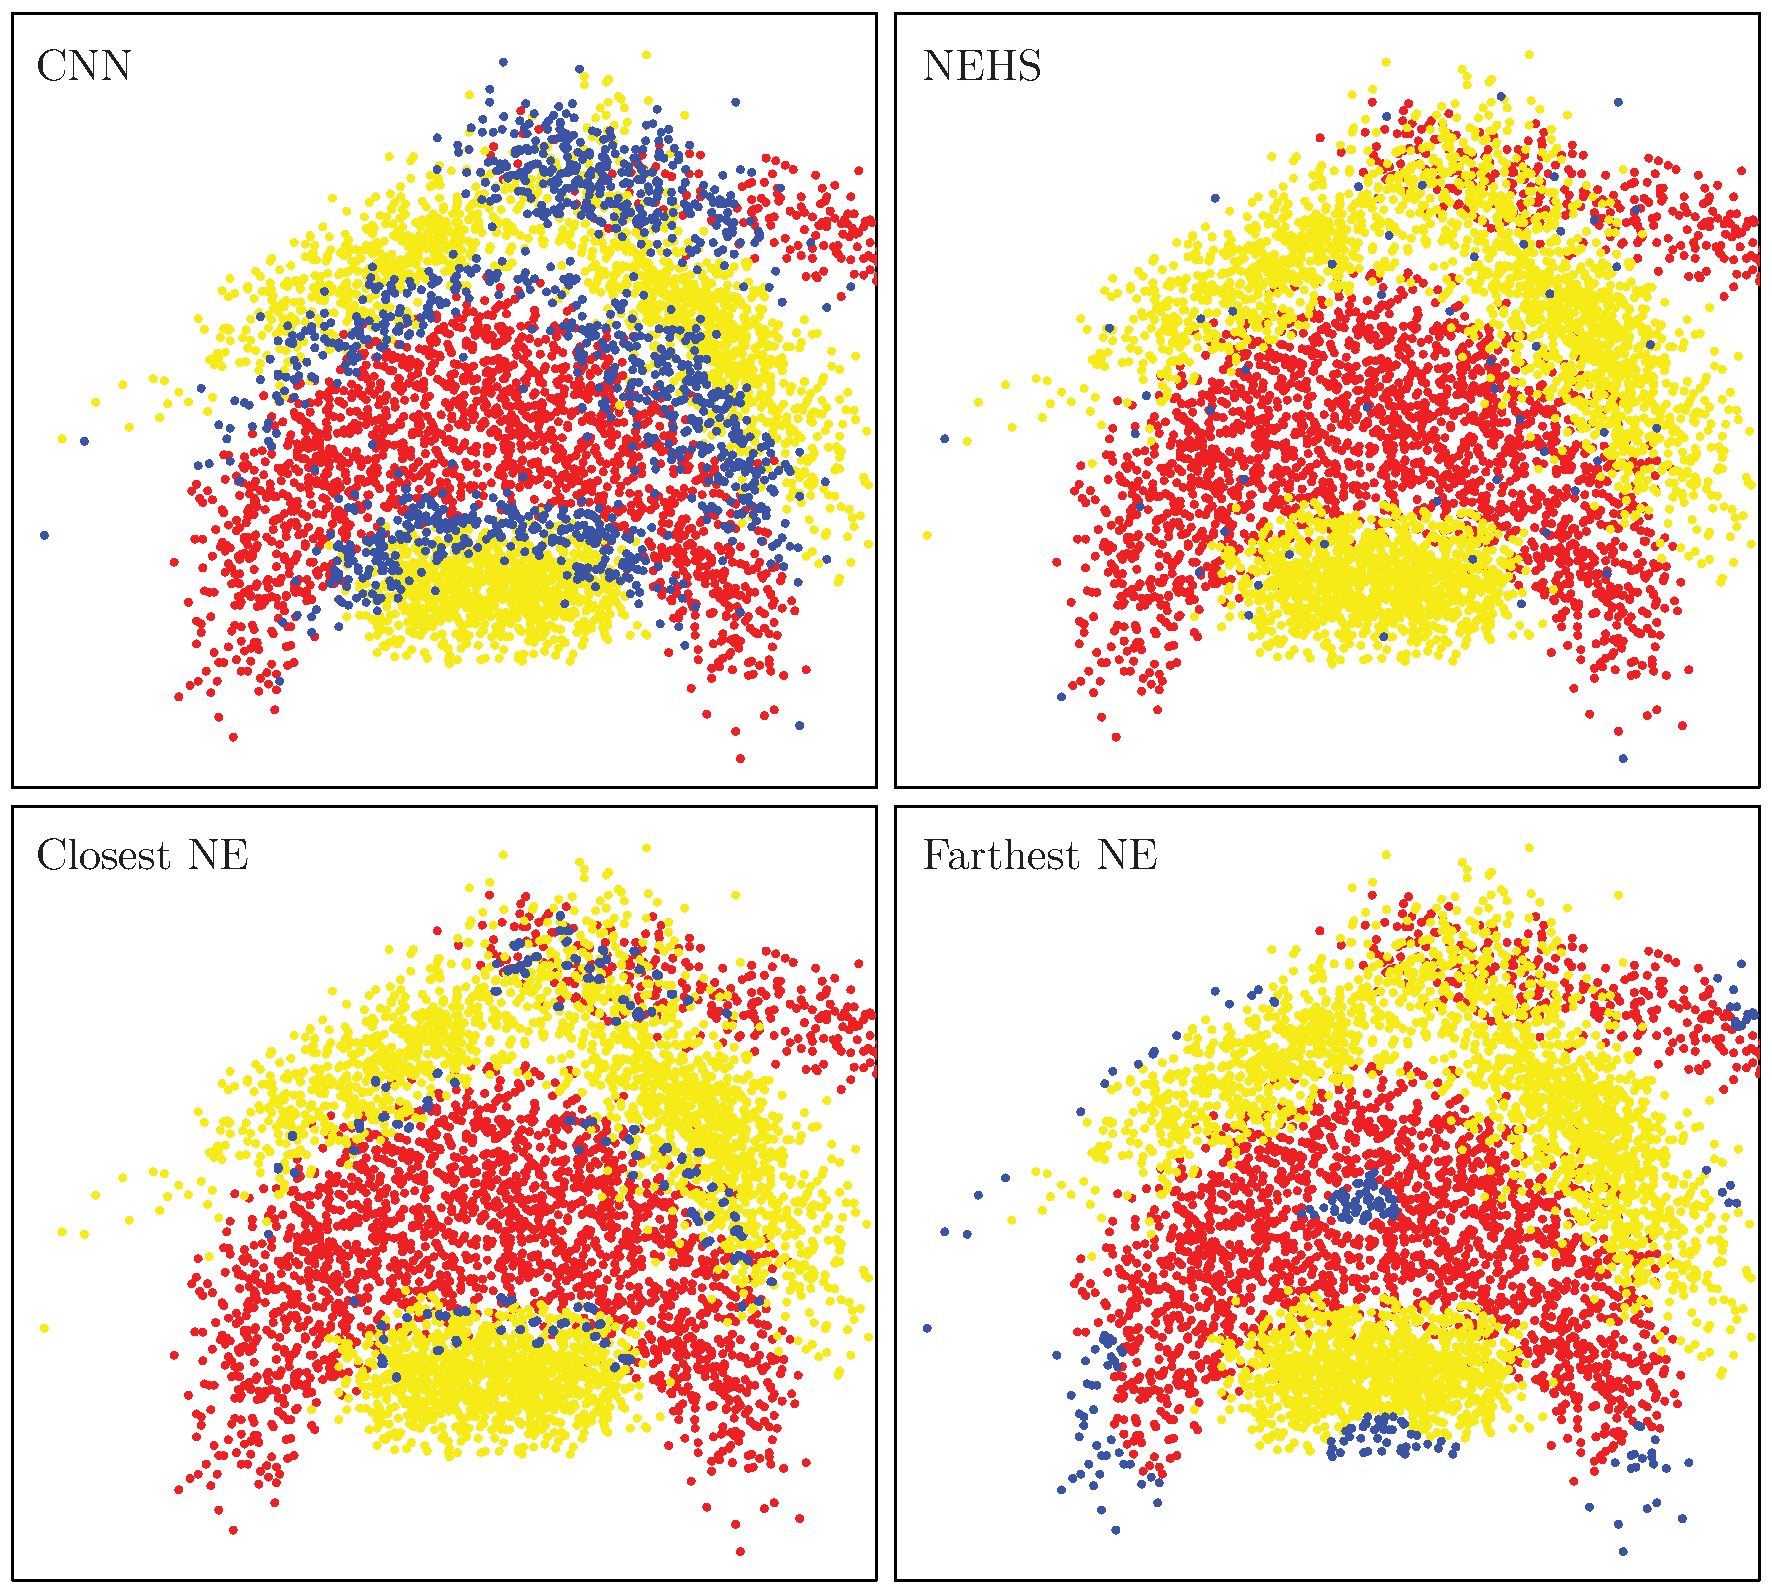
\includegraphics[width=0.8\textwidth]{seleccion.pdf}
\caption[Algoritmos de Selección de Instancias]{Subconjunto de instancias seleccionadas por CNN, NEHS, Closest NE y Farthest NE, para el conjunto de instancias \textsc{Banana}. Las instancias están pintadas en amarillo y rojo según su clase en el conjunto de datos, y en azul aquellas instancias pertenecientes a la selección correspondiente.}
\label{seleccion}
\end{figure}

\subsubsection{Condensed Nearest Neighbor}

Descrito por \emph{Hart} \cite{Hart:2006:CNN:2263267.2267647}, CNN 

\begin{algorithm}
\caption{Condensed Nearest Neighbor}
\label{cnn-alg}
\begin{algorithmic}[1]

\Require $T$ conjunto de instancias inicial
\Ensure Conjunto de instancias $R \subseteq T$

\State $R \gets \left\lbrace \mathrm{Una\ instancia\ cualquiera}\ t \in T \right\rbrace$
\Repeat
	\State $R' \gets R$
	\ForAll{$t \in T$}
		\If{$t$ es mal clasificada usando $R$ con un clasificador 1-NN}
			\State $R \gets R \cup \left\lbrace t \right\rbrace$
		\EndIf
	\EndFor
\Until{$R = R'$}
\State \Return{$R$}
\end{algorithmic}
\end{algorithm}

\subsubsection{Nearest Enemy Hypersphere Selection}

La idea tras el uso de la regla NN es que instancias ``cercanas'' en un espacio cualquiera (\emph{i.e.} con atributos similares) comparten su clasificación; esto conlleva a la división de dicho espacio en regiones con instancias de igual clase. La idea fundamental de \emph{Nearest Enemy Hypersphere Selection} (NEHS) es seleccionar instancias en los centros de dichas regiones, con la finalidad de reducir la cantidad de instancias necesarias para generalizar el espacio descrito por el conjunto original. Para esto hace uso de la distancia del \emph{enemigo más cercano}: cada instancia $t \in T$ tiene un enemigo más cercano $\mathrm{NE}(t)$, cuya distancia $\varphi(t,\mathrm{NE}(t))$ define una hiperesfera en el espacio dentro de la cual toda instancia comparte la clase $\omega_t$. NEHS implementa una estrategia \emph{greedy} que busca seleccionar las mayores hiperesferas que no intersecten entre sí. Ver algoritmo \ref{necs-alg}.

\begin{algorithm}
\caption{Nearest Enemy Hypersphere Selection}
\label{necs-alg}
\begin{algorithmic}[1]

\Require $T$ conjunto de instancias inicial, $\Delta$ porcentaje de instancias a excluir
\Ensure Conjunto de instancias $R \subseteq T$

\State $R \gets \emptyset$
\ForAll{$t \in T$ en orden descendiente de distancia NE\par
	\hskip\algorithmicindent excluyendo las últimas $\Delta\vert T \vert$ instancias}
	\If{$\lnot\exists\ r \in R$ tal que $\varphi(t,r) < \varphi(r,\mathrm{NE}(r)) + \varphi(t,\mathrm{NE}(t))$}
		\State $R \gets R \cup \left\lbrace t \right\rbrace$
	\EndIf
\EndFor
\State \Return{$R$}
\end{algorithmic}
\end{algorithm}

\subsubsection{Closest Nearest Enemy}

La distancia del \emph{enemigo más cercano} (NE) de una instancia cualquiera $t \in T$ (\emph{i.e.} $\varphi(t,\mathrm{NE}(t))$), indica su cercanía a los bordes de decisión establecidos mediante un clasificador 1-NN. La selección por \emph{Closest NE} escoge aquellas instancias con \emph{menor} distancia NE entre las instancias en $T$, \emph{i.e.} instancias pertenecientes --o cercanas-- a los bordes de decisión de los datos. En el presente trabajo, \emph{Closest NE} selecciona el $5\%$ ($\delta = 0.05$) de instancias con menor distancia NE.

\begin{equation}
R_\mathrm{ClosestNE} = \left\lbrace \delta \vert T \vert\ \mathrm{instancias\ con\ menor\ distancia\ NE} \right\rbrace
\end{equation}

\subsubsection{Farthest Nearest Enemy}

Similar a la selección por \emph{Closest NE}, \emph{Farthest NE} se basa en el uso de la distancia NE para incluir instancias en el conjunto reducido $R \subseteq T$. Sin embargo, \emph{Farthest NE} selecciona aquellas instancias con \emph{mayor} distancia NE, \emph{i.e.} instancias alejadas de los bordes de decisión y cercanas a los centros de sus respectivas regiones. Este método también usa un porcentaje de selección igual al $5\%$ ($\delta = 0.05$) de las instancias en $T$.

\begin{equation}
R_\mathrm{FarthestNE} = \left\lbrace \delta \vert T \vert\ \mathrm{instancias\ con\ mayor\ distancia\ NE} \right\rbrace
\end{equation}

\section{Modificaciones particulares}

\subsection{Adaptación de GGA, SGA y CHC}

Para aplicar algún algoritmo genético al problema de \emph{SI}, es necesario describir las estrategias de selección, recombinación, mutación y reemplazo que seguirá el algoritmo durante el proceso evolutivo.

GGA, SGA y CHC requieren de un operador que seleccione individuos de la población para participar en el proceso reproductivo. Se emplea el método de \emph{selección por torneo} en su versión ``determinista'': se escoge al azar un conjunto de individuos entre la población original, y es seleccionado el más apto entre ellos. El tamaño de dicho conjunto debe ser pequeño; generalmente se usa un ``tamaño de torneo'' entre 2 y 5 \cite{Miller95geneticalgorithms}. En este trabajo se usan torneos de tamaño 3.

Debido a que CHC aplica un operador de recombinación particular (HUX) y no requiere de un operador de mutación, dichos operadores deben ser definidos solo para GGA y SGA. El operador de \emph{crossover} aplicado en ambos algoritmos es el \emph{recombinación en un punto}. Dados dos cromosomas ``padres'', se elige aleatoriamente un punto de corte en la longitud de ambos cromosomas; los cromosomas ``hijos'' resultan de combinar la sección izquierda del corte de un padre, con la sección derecha del corte del otro padre. El operador de mutación sigue --en ambos casos-- el esquema estándar de modificación de cada bit con una cierta probabilidad.

Finalmente, es necesario describir los criterios de reemplazo. Al tratarse de estrategias evolutivas generacionales, GGA y CHC reemplazan la población de forma incondicional en favor de la decendencia. En cambio, el criterio de reemplazo usado en SGA es ``elitista''; se sustituyen los peores individuos en la población por la nueva decendencia generada, solo si dicha decendencia es mejor.

\subsection{Adaptación de PBIL}

La estrategia evolutiva de PBIL no requiere modificaciones adicionales para su aplicación al problema de selección de instancias; está diseñado para encontrar soluciones con representación binaria, lo que permite su aplicación directa al problema. La única modificación realizada al esquema estándar de PBIL es en el método de generación del vector de probabilidades iniciales, reflejando lo descrito en la sección \ref{generacion-sol-inic}.

\subsection{Adaptación de PSO}

La adaptación de PSO al problema de \emph{SI} es mayor, debido a que PSO está pensado para problemas con representación en espacios euclideanos; \emph{i.e.} es necesario el mapeo de vectores en $\mathbb{R}^l$ a soluciones con representación binaria. En este sentido, se adopta el esquema poblacional de PBIL en el que el genotipo de la población se representa de forma probabilística.

A esta adaptación de PSO la llamaremos \emph{Population-Based PSO} (ver algoritmo \ref{pbpso-alg}), en la cuál el vector de posición $\vec{X_i}$ de cada partícula es un vector de probabilidades que representa el genotipo de una población particular. Esto permite la generación de soluciones en codificación binaria para su respectiva evaluación, en base al vector de probabilidades que describe dicha población. A diferencia del PSO tradicional, la selección de óptimos locales y globales se hace en base a las soluciones generadas mediante $\vec{X_i}$, y no en base al vector $\vec{X_i}$ por si solo. Sin embargo, la modificación de los vectores de probabilidad y velocidad ($\vec{X_i}$ y $\vec{V_i}$ respectivamente) sigue la estrategia de actualización estándar en base a la mejor solución local y la mejor solución global.

\begin{algorithm}
\caption{Population-Based PSO}
\label{pbpso-alg}
\begin{algorithmic}[1]

\Require \texttt{pop} tamaño de la población,
	\texttt{part} número de particulas,
	\texttt{vmax} velocidad máxima,
	\texttt{w} peso de inercia,
	\texttt{c1} peso del mejor local,
	\texttt{c2} peso del mejor global
\Ensure Una solución al problema

\For{$i \in [1 \dots \texttt{part}]$}
	\State{$\vec{X_i} \gets$ Vector de probabilidades de tamaño $l$}
	\State{$\vec{V_i} \gets$ Vector de velocidades aleatorias entre $[-\texttt{vmax},\texttt{vmax}]$}
	\State{$p_i \gets$ Generar una solución a partir de $\vec{X_i}$}
\EndFor
\State $s^* \gets$ La \emph{mejor} solución $p_i, i \in [1 \dots \texttt{part}]$
\While {$\neg$ Condición de parada}
	\For{$i \in [1 \dots \texttt{part}]$}
		\State{$\vec{X_i} \gets \vec{X_i} + \vec{V_i}$}
		\State{Limitar valores en $\vec{X_i}$ entre $[0,1]$}
		\State{$\vec{V_i} \gets \texttt{w} \vec{V_i} + \texttt{c1}\ \mathrm{Unif}(0,1) (p_i - \vec{X_i}) + \texttt{c2}\ \mathrm{Unif}(0,1) (s^* - \vec{X_i})$}
		\State{Limitar valores en $\vec{V_i}$ entre $[-\texttt{vmax},\texttt{vmax}]$}
		\State{$P \gets$ Generar población de tamaño \texttt{pop} a partir de $\vec{X_i}$}
		\If {El \emph{mejor} individuo en $P$ es \emph{mejor} que $p_i$}
			\State $p_i \gets$ El \emph{mejor} individuo en $P$
			\If {$p_i$ es \emph{mejor} que $s^*$}
				\State $s^* \gets p_i$
			\EndIf
		\EndIf
	\EndFor
\EndWhile
\State \Return $s^*$

\end{algorithmic}
\end{algorithm}

Esta versión de PSO puede clasificarse como una metaheurística de la clase de \emph{Algorítmos de Coevolución Cooperativa} \cite{Derrac:2009:FSU:1574827.1574906} (puesto que mantiene diferentes poblaciones que evolucionan de forma colaborativa) y \emph{Algoritmos de Estimación de Distribución} (debido a que adopta las ideas de representación descritas por PBIL).

\chapter{Evaluación Experimental}
\label{capitulo4}
\lhead{Capítulo 4. \emph{Evaluación Experimental}}

Este capítulo consiste en la descripción del diseño experimental empleado durante la evaluación de los métodos introducidos en los capítulos anteriores, así como el análisis de los resultados obtenidos de dicha evaluación. El objetivo de este estudio radica en la comparación empírica de cinco metaheurísticas (\emph{i.e.} GGA, SGA, CHC, PBIL y PSO) adaptadas para encontrar soluciones al problema de selección de instancias. Adicionalmente, se pretende estudiar el impacto de la aplicación de estrategias alternativas de generación de soluciones iniciales: disminuyendo la probabilidad de aparición de cada bit (de $50\%$ a $5\%$) y modificando dichas probabilidades en función de los subconjuntos de instancias generados por diferentes algoritmos heurísticos (\emph{i.e.} CNN, NEHS, Closest NE y Farthest NE).

\section{Diseño Experimental}

El diseño experimental aplicado permite establecer la efectividad de las metaheurísticas descritas en función de
\begin{inparaenum}[\itshape a\upshape)]
\item la reducción del conjunto de instancias usado para el entrenamiento del clasificador (en este caso un clasificador 1-NN), y
\item la precisión de dicho clasificador --una vez entrenado-- al clasificar instancias desconocidas.
\end{inparaenum}
La metodología experimental debe permitir la generalización del comportamiento de las metaheurísticas, así como las estrategias de generación de soluciones iniciales, con la finalidad de comparar los resultados obtenidos y establecer los métodos más efectivos frente al problema de selección de instancias.

\subsection{Conjuntos de datos}
\label{data-section}

Un factor esencial en la evaluación de métodos de selección de instancias es el conjunto de datos utilizado; la distribución de los datos, el número de instancias y atributos, y la cantidad de datos ruidosos, son solo algunos de los elementos que modifican el espacio de búsqueda del problema y por ende la efectividad de los algoritmos heurísticos para encontrar buenas soluciones. Los conjuntos de datos usados en este trabajo pertenecen al \emph{UCI Machine Learning Repository} \cite{BacheLichman:2013} y al \emph{KEEL Data-Mining Software Tool} \cite{alcala2010keel}.

Los 14 conjuntos seleccionados fueron separados en 3 grupos en función del número de instancias de cada conjunto. En la tabla \ref{data-small} se presentan 9 conjuntos con menor cantidad de instancias.

\begin{table}[h!]
\centering
\begin{tabular}{l c c c}
\hline
\textsc{Conjunto} & \textsc{Instancias} & \textsc{Atributos} & \textsc{Clases} \\
\hline
\hline
Cleveland & 297 & 13 &  5 \\
Glass     & 214 &  9 &  7 \\
Iris      & 150 &  4 &  3 \\
Led7Digit & 500 &  7 & 10 \\
Monk      & 432 &  6 &  2 \\
Pima      & 768 &  8 &  2 \\
WDBC      & 569 & 30 &  2 \\
Wine      & 178 & 13 &  3 \\
Wisconsin & 683 &  9 &  2 \\
\hline
\end{tabular}
\caption{Conjuntos de datos pequeños}
\label{data-small}
\end{table}

En la tabla \ref{data-med} se describen dos conjuntos de datos caracterizados como de tamaño medio.

\begin{table}[h!]
\centering
\begin{tabular}{l c c c}
\hline
\textsc{Conjunto} & \textsc{Instancias} & \textsc{Atributos} & \textsc{Clases} \\
\hline
\hline
Banana       &  5300 &  2 &  2 \\
Segmentation &  2100 & 19 &  7 \\
\hline
\end{tabular}
\caption{Conjuntos de datos medianos}
\label{data-med}
\end{table}

Finalmente, los 3 conjuntos con mayor número de instancias se presentan en la tabla \ref{data-big}.

\begin{table}[h!]
\centering
\begin{tabular}{l c c c}
\hline
\textsc{Conjunto} & \textsc{Instancias} & \textsc{Atributos} & \textsc{Clases} \\
\hline
\hline
Penbased    & 10992 & 16 & 10 \\
Satimage     &  6435 & 36 &  6 \\
Thyroid      &  7200 & 21 &  3 \\
\hline
\end{tabular}
\caption{Conjuntos de datos grandes}
\label{data-big}
\end{table}

\subsection{Particiones y ejecuciones}

Los conjuntos de datos considerados en la sección anterior son particionados usando la estrategia de validación cruzada en 10 grupos (10-\emph{fold cross-validation}). El conjunto inicial de instancias $T$ es dividido en 10 subconjuntos disjuntos de igual tamaño $T_1, T_2, \dots T_{10}$. Cada conjunto $T_i$ mantiene la proporción de distribución de las clases del conjunto original $T$. En función de esta partición, se definen los pares de conjuntos $(T'_i, T_i)$, con $i = 1 \dots 10$, donde $T'_i = T \setminus T_i$.

El conjunto $T'_i$, también conocido como el conjunto de ``entrenamiento'', es usado por las metaheurísticas durante el proceso de búsqueda para evaluar soluciones intermedias, en vez de usar $T$. %, se usa el conjunto $T'_i$ como el conjunto de instancias inicial.
Las instancias restantes (pertenecientes al conjunto $T_i$) son usadas como conjunto de ``validación'', \emph{i.e.} la mejor solución encontrada durante la ejecución, es usada para clasificar las instancias desconocidas de $T_i$.

En base a esta estrategia, se definen los criterios de comparación empleados en el presente trabajo. Dada una solución $R \subseteq T'_i$ al problema de SI encontrada por una metaheurística, se considera:

\begin{itemize}
\item \emph{Error de Entrenamiento}\\
El porcentaje de instancias en $T'_i$ mal clasificadas usando $R$ como conjunto de prototipos en un clasificador 1-NN. Para el cálculo de esta métrica no se remueven las instancias antes de ser clasificadas (\emph{Leave-one-out cross-validation}), por lo que toda instancia en $R$ se considera correctamente clasificada.
\item \emph{Error de Validación}\\
El porcentaje de instancias en $T_i$ mal clasificadas usando $R$ como conjunto de prototipos en un clasificador 1-NN.
\item \emph{Tamaño}\\
El tamaño de $R$ en función de $T'_i$ (\emph{i.e.} $\frac{100 \vert R \vert}{\vert T'_i \vert}$).
\item \emph{Tiempo}\\
Segundos empleados por el algoritmo durante la búsqueda.
\end{itemize} 

Cada metaheurística es evaluada usando los 10 pares de conjuntos $(T'_i, T_i)$. Por cada par de conjunto entrenamiento-validación se realizan 3 repeticiones. \emph{i.e.} un total de 30 ejecuciones de una metaheurística para un conjunto de datos y un tipo de inicialización particular. Las ejecuciones fueron realizadas de manera independiente en máquinas de tipo \texttt{c3.2xlarge} de \emph{Amazon EC2}, que disponen de 8 CPUs Intel Xeon E5-2680 v2 (Ivy Bridge), 15GB de memoria RAM y 80GB de disco duro de estado sólido. Todos los experimentos se realizaron bajo el sistema operativo Amazon Linux AMI 2014.03.2 y utilizando GCC 4.8.2.

\subsection{Parámetros}
\label{sec-parametros}

Cada metaheurística depende de un conjunto de parámetros que regulan el proceso de búsqueda sobre el espacio de posibles soluciones. El valor de cada parámetro y la interacción entre ellos, determinan el comportamiento del algoritmo y su capacidad para encontrar buenas soluciones. Sin embargo, los valores que indican el buen comportamiento de una metaheurística, son altamente dependientes del problema en general, e incluso de la instancia particular que se pretenda evaluar. Esto lo convierte en un proceso complejo, que a menudo conlleva a un diseño factorial con el fin de estudiar la influencia de los parámetros y sus interacciones en asegurar la calidad de las soluciones obtenidas.

En el presente trabajo se realizó la entonación de las metaheurísticas seleccionadas en los capítulos anteriores. Los resultados obtenidos de este proceso se describen en el Apéndice \ref{apendiceA}. En la tabla \ref{table-parameters} se presentan los parámetros seleccionados para cada metaheurística.

\begin{table}[h!]
\centering
\begin{tabular}{l c c c c c}
\hline
\multirow{2}{*}{\textsc{Parámetros}}
	& \multicolumn{5}{c}{\textsc{Algoritmos}} \\\cline{2-6}
	& GGA & SGA & CHC & PBIL & PSO \\
\hline
\hline
Iteraciones        &  1000 &  1000 &  1000 &  1000 &  1000 \\
Población          &    50 &    30 &    30 &    40 &     5 \\
Prob. de Cruce     &   0.9 &   1.0 &     - &     - &     - \\
Prob. de Mutación  & 0.001 & 0.001 &     - & 0.001 &     - \\
Mutation Shift     &     - &     - &     - &  0.01 &     - \\
Learning Rate      &     - &     - &     - &   0.1 &     - \\
Neg. Learning Rate &     - &     - &     - &  0.01 &     - \\
Partículas         &     - &     - &     - &     - &     5 \\
Velocidad Máxima   &     - &     - &     - &     - &   0.2 \\
Inercia            &     - &     - &     - &     - &   0.9 \\
c1                 &     - &     - &     - &     - &   0.1 \\
c2                 &     - &     - &     - &     - &   0.1 \\
\hline
\end{tabular}
\caption{Parámetros usados en cada metaheurística}
\label{table-parameters}
\end{table}

\subsection{Tablas de resultados}

En la sección \ref{sec-res} son presentados y analizados los resultados obtenidos del proceso experimental. Las tablas de resultados deben permitir identificar las mejores estrategias de inicialización o las mejores metaheurísticas, según corresponda.

En primer lugar, se presenta una tabla con los resultados promedio de cada metaheurística, en función de los 4 criterios de comparación descritos en la subsección \ref{sec-parametros}. Para una metaheurística particular, se promedian sus resultados para los conjuntos de datos que correspondan.

Sin embargo, al promediar los resultados puede perderse información relevante, puesto que el comportamiento de una metaheurística depende del conjunto de datos que se use para evaluarla. Por esta razón, se introducen las tablas de ranking, que presentan información adicional que permite comparar las metaheurísticas bajo un mismo contexto. Por cada conjunto de datos, las metaheurísticas son rankeadas de acuerdo a sus resultados en una métrica particular. A partir del ordenamiento en cada conjunto de datos, la tabla muestra el ranking promedio de cada metaheurística y el número de veces que logró el mejor resultado. Estos valores son calculados usando las métricas de tamaño, error de validación y la combinación lineal de ambos.

Ambas tablas son usadas para presentar los resultados por cada estrategia de inicialización. Para la primera tabla, se promedian los resultados no solo por conjunto de datos, sino también por metaheurística. Para las tablas de ranking ocurre lo mismo: los ordenamientos son realizados por cada combinación de metaheurística y conjunto de datos evaluados.

\section{Resultados}
\label{sec-res}

En esta sección se presentan los resultados obtenidos durante la evaluación experimental. En la sección \ref{sec-comp-inits} se comparan diferentes estrategias de inicialización de soluciones con representación binaria,
\begin{inparaenum}[\itshape a\upshape)]
\item evaluando el impacto de disminuir la probabilidad de aparición de bits, y
\item modificando la distribución de dicha probabilidad a lo largo de la cadena de bits, de una distribución uniforme a una distribución personalizada basada en los conjuntos seleccionados por algoritmos heurísticos al problema de SI.
\end{inparaenum}
Una vez seleccionada la mejor estrategia de inicialización, en la sección \ref{sec-comp-meta} se comparan los resultados obtenidos por las 5 metaheurísticas descritas. Se concluye con un estudio que busca determinar (en caso que existan) aquellas metaheurísticas que se comporten consistentemente mejor que el resto.

\subsection{Comparación entre inicializaciones}
\label{sec-comp-inits}

Bajo el contexto del problema de SI, modificar la estrategia de inicialización de soluciones tiene un objetivo claro: iniciar el proceso de búsqueda en ``buenas'' soluciones. Una buena solución al problema de SI debe minimizar tanto la cardinalidad del conjunto $R$, como el error de clasificación usando $R$ como conjunto de prototipos. En este sentido, se propone disminuir la probabilidad de aparición de bits $\delta$ para reducir la cardinalidad de soluciones iniciales, y modificar la distribución de dicha probabilidad, beneficiando a instancias seleccionadas por diferentes algoritmos heurísticos, con la intensión de reducir el error de clasificación.

Con la finalidad de comparar diferentes estrategias de inicialización, se realizaron experimentos sobre los conjuntos de datos grandes (Tabla \ref{data-big}). Los resultados obtenidos son presentados y analizados a continuación.

\subsubsection{Probabilidad de aparición de bit}

Con la finalidad de reducir la cardinalidad de las soluciones iniciales generadas, en un intento de reducir el número de iteraciones necesarias para conseguir porcentajes de reducción aceptables, este estudio propone la reducción de la probabilidad de aparición de bits $\delta$. En esta sección se estudia el impacto de la disminución propuesta, usando 3 posibles valores: $50\%$, $25\%$ y $5\%$.

En la tabla \ref{table-unif} se presentan los resultados promedio de la evaluación de las 5 metaheurísticas sobre los conjuntos de datos grandes, modificando únicamente el parámetro $\delta$ (probabilidad de aparición de bit).

\begin{table}[h!]
\centering
\begin{tabular}{c c c c c}
\hline
\multirow{2}{*}{$\delta$}
	& \multirow{2}{*}{\textsc{Tiempo}}
	& \multirow{2}{*}{\textsc{Tamaño}}
	& \multicolumn{2}{c}{$\%$ de \textsc{Error}} \\\cline{4-5}
 & & & \scriptsize{Entrenamiento} & \scriptsize{Validación} \\
\hline
\hline
$50\%$ & 1324.96 & 37.09 & \textbf{2.94} & \textbf{6.60} \\
$25\%$ & 1193.26 & 19.83 & 4.14 & 6.71 \\
$5\%$  & \textbf{893.24} & \textbf{4.67} & 6.25 & 7.28 \\
\hline
\end{tabular}
\caption[Resultados modificando la probabilidad de aparición de bit]{Resultados promedio de las 5 metaheurísticas\\frente a los conjuntos de datos grandes, usando una\\probabilidad de aparición de bit $\delta$ igual a $50\%$, $25\%$ y $5\%$.}
\label{table-unif}
\end{table}

Estos datos corroboran la hipótesis de que al usar $\delta = 50\%$, es necesario un mayor número de iteraciones para converger a soluciones con porcentajes de reducción aceptables \cite{cano2003using}. Como era de esperarse, la disminución del parámetro $\delta$ implica una reducción similar en términos del tamaño de las soluciones encontradas. Esto a su vez, supone una disminución importante en el tiempo de ejecución de los algoritmos, debido a que la evaluación de soluciones intermedias depende en gran medida de la cardinalidad de dichas soluciones.

\begin{figure}[h!]
\centering
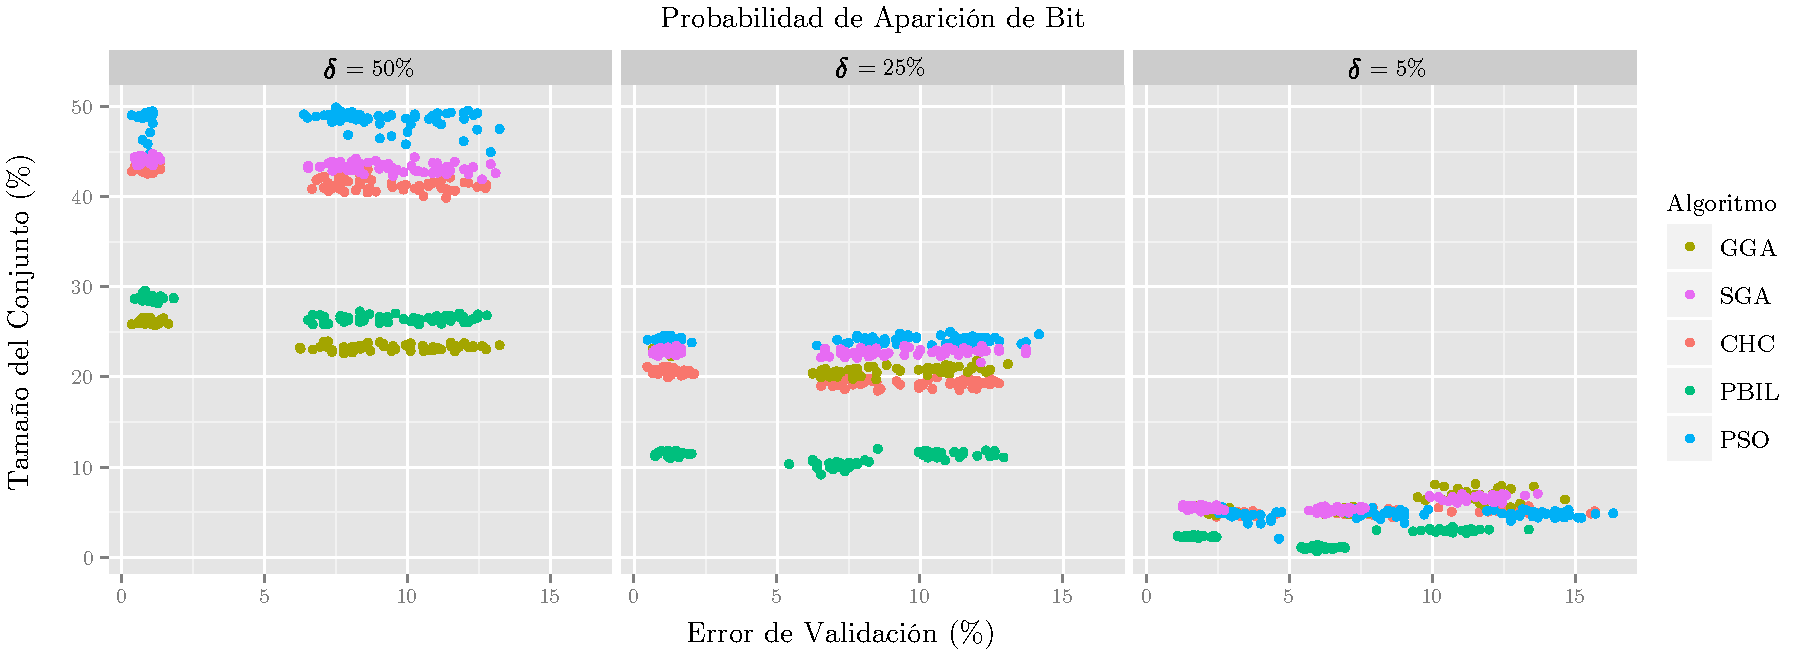
\includegraphics[width=\textwidth]{uniforme.pdf}
\caption[Tamaño \emph{vs} error de validación modificando $\delta$]{Tamaño del conjunto \emph{vs} error de validación en\\ejecuciones de las metaheurísticas usando $\delta$ igual a $50\%$, $25\%$ y $5\%$.}
\label{fig-unif}
\end{figure}

En la figura \ref{fig-unif} resultan evidentes las diferencias en el tamaño de las soluciones encontradas usando las 3 probabilidades seleccionadas. No es únicamente una diferencia promedio: la inicialización usando $\delta = 5\%$ logra que las 5 metaheurísticas consigan soluciones más consistentes en términos de reducción.

Sin embargo, la disminución del parámetro $\delta$ conlleva a un aumento en los errores de entrenamiento y validación. No obstante, en ambos casos los errores se mantienen en valores aceptables, y en el caso del error de validación, la diferencia es poco significativa.

\begin{table}[h!]
\centering
\begin{tabular}{c c c|c c c|c c c}
\hline
\multicolumn{3}{c|}{\textsc{Error de Validación}}
	& \multicolumn{3}{c|}{\textsc{Tamaño}}
	& \multicolumn{3}{c}{\textsc{Error + Tamaño}} \\
\hline
$\delta$ & Rank & Mejor & $\delta$ & Rank & Mejor & $\delta$ & Rank & Mejor \\
\hline
\hline
$50\%$ & 1.73 & 9 & $5\%$  & 1.0 & 15 & $5\%$  & 1.0 & 15 \\
$25\%$ & 1.93 & 4 & $25\%$ & 2.0 &  0 & $25\%$ & 2.0 &  0 \\
$5\%$  & 2.33 & 2 & $50\%$ & 3.0 &  0 & $50\%$ & 3.0 &  0 \\
\hline
\end{tabular}
\caption[Ranking de probabilidad de bit $\delta$ según el tamaño y error de validación]{Ranking de inicializaciones según el tamaño y error de validación, considerando los promedios de las ejecuciones de cada algoritmo frente a los conjuntos de datos grandes. Por cada inicialización, se presenta su ranking promedio (\emph{Rank}) y el número de veces que obtuvo los mejores resultados (\emph{Mejor}).}
\label{table-unif-rank}
\end{table}

A pesar de que las diferencias en el error de validación favorecen el uso de\linebreak$\delta = 50\%$, la disminución de la probabilidad de aparición de bit al $5\%$ supone beneficios importantes en relación a la reducción alcanzada (ver la tabla \ref{table-unif-rank}) y al tiempo de ejecución. Por esta razón, se decidió usar $\delta = 5\%$ durante el resto de la evaluación experimental.

\subsubsection{Inicialización usando algoritmos heurísticos}

En esta sección se evalua el impacto de generar soluciones iniciales, modificando la distribución de probabilidad a lo largo la cadena de bits que representa una solución al problema de SI. El enfoque estandar emplea una distribución uniforme con probabilidad $\delta$, \emph{i.e.} todos los bits tienen igual probabilidad de estar ``prendidos''. En el presente trabajo empleamos una técnica de modificación de distribución, basada en la selección realizada por algoritmos heurísticos.

\begin{table}[h!]
\centering
\begin{tabular}{l c c c c}
\hline
\multirow{2}{*}{\textsc{Inicialización}}
	& \multirow{2}{*}{\textsc{Tiempo}}
	& \multirow{2}{*}{\textsc{Tamaño}}
	& \multicolumn{2}{c}{$\%$ de \textsc{Error}} \\\cline{4-5}
 & & & \scriptsize{Entrenamiento} & \scriptsize{Validación} \\
\hline
\hline
Uniforme   & \textbf{893.24} & \textbf{4.67} & 6.25 & \textbf{7.28} \\
NEHS       & 958.94 & 4.70 & \textbf{6.20} & \textbf{7.28} \\
CNN        & 921.68 & 5.11 & 6.27 & 7.85 \\
FarthestNE & 932.19 & 4.98 & 6.94 & 7.67 \\
ClosestNE  & 932.75 & 5.56 & 7.21 & 8.95 \\
\hline
\end{tabular}
\caption[Resultados usando distribuciones uniforme y heurísticas]{Resultados promedio de las 5 metaheurísticas frente a los\\conjuntos de datos grandes, usando distribuciones de probabilidad\\uniforme y basadas en algoritmos heurísticos.}
\label{table-inits}
\end{table}

En la tabla \ref{table-inits} se presentan los resultados promedio del usar una distribución uniforme y distribuciones basadas en CNN, NEHS, Closest NE y Farthest NE, para la generación de soluciones iniciales en las 5 metaheuristicas descritas. Los datos en tiempo de ejecución son previsibles, debido al tiempo añadido de encontrar soluciones mediante el uso de estos algoritmos heurísticos. Sin embargo, contrario a lo esperado, estas modificaciones no mejoran significativamente los porcentajes de error obtenidos mediante una distribución uniforme. Más aún, CNN, Closest NE y Farthest NE empeoran los resultados en todos los aspectos. Solo NEHS reporta resultados alentadores, en el que mejora el error de entrenamiento e iguala el error de validación frente a una distribución uniforme.

La figura \ref{fig-inits} confirma los aspectos señalados: el comportamiento de inicializaciones basadas en CNN, Closest NE y Farthest NE difieren significativamente del comportamiento de aquellas basadas en NEHS o una distribución uniforme. Estas últimas (NEHS y Uniforme) muestran un comportamiento similar en función de ambos objetivos del problema.

\begin{figure}[h!]
\centering
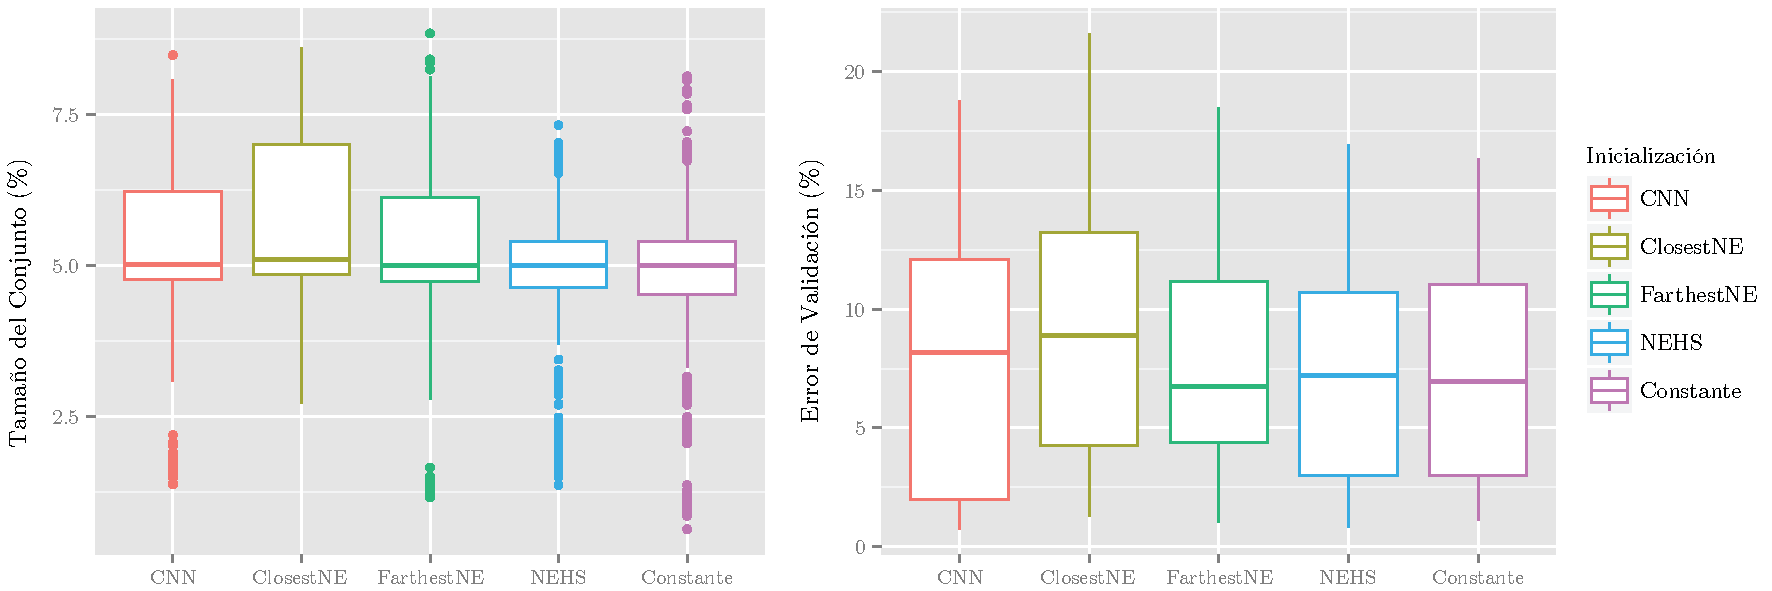
\includegraphics[width=\textwidth]{inits-boxplot.pdf}
\caption[Tamaño y error de validación usando algoritmos heurísticos]{Diagramas de caja del tamaño y error de validación usando distribuciones de probabilidad uniforme y basadas en algoritmos heurísticos.}
\label{fig-inits}
\end{figure}

Sin embargo, la tabla \ref{table-inits-rank} sugiere que una inicialización basada en NEHS resulta conveniente en función de los dos objetivos del problema, siendo el que presenta mejor ranking promedio en base al error de validación y a la combinación lineal entre el error y el tamaño del conjunto seleccionado. En función de estos resultados, se usa NEHS como heurística de inicialización de las ejecuciones realizadas en la sección \ref{sec-comp-meta}, cuya finalidad es determinar aquellas metaheurísticas que se comporten consistentemente mejor que las demás.

\begin{table}[h!]
\centering
\begin{tabular}{l c c|l c c|l c c}
\hline
\multicolumn{3}{c|}{\textsc{Error de Validación}}
	& \multicolumn{3}{c|}{\textsc{Tamaño}}
	& \multicolumn{3}{c}{\textsc{Error + Tamaño}} \\
\hline
Inicialización & Rank & Mejor & Inicialización & Rank & Mejor & Inicialización & Rank & Mejor \\
\hline
\hline
NEHS       & 2.06 & 4 & Uniforme   & 1.86 & 6 & NEHS       & 2.00 & 5 \\
Uniforme   & 2.40 & 2 & NEHS       & 2.26 & 3 & Uniforme   & 2.20 & 2 \\
CNN        & 2.86 & 4 & FarthestNE & 2.86 & 4 & CNN        & 2.93 & 4 \\
FarthestNE & 2.93 & 5 & CNN        & 3.60 & 2 & FarthestNE & 3.06 & 4 \\
ClosestNE  & 4.73 & 0 & ClosestNE  & 4.40 & 0 & ClosestNE  & 4.80 & 0 \\
\hline
\end{tabular}
\caption[Ranking de inicializaciones según el tamaño y error de validación]{Ranking de inicializaciones según el tamaño y error de validación, considerando los promedios de las ejecuciones de cada algoritmo frente a los conjuntos de datos grandes. Por cada inicialización, se presenta su ranking promedio (\emph{Rank}) y el número de veces que obtuvo los mejores resultados (\emph{Mejor}).}
\label{table-inits-rank}
\end{table} 

\subsection{Comparación entre metaheurísticas}
\label{sec-comp-meta}

Para controlar el proceso de búsqueda, cada metaheurística emplea técnicas diversas para recorrer el espacio de posibles soluciones. Su capacidad para encontrar buenas soluciones está íntimamente ligado al problema que se desea resolver, la representación de sus soluciones, la función de objetivo, entre otros factores. La distribución del espacio de búsqueda puede alterar significativamente la efectividad de una metaheurística particular. Por esta razón, al estudiar el comportamiento de diferentes metaheurísticas frente al problema de SI, es necesario identificar aquellas metaheurísticas que exiban mejor capacidad para seleccionar subconjuntos de instancias que cumplan con los objetivos planteados por el problema.

A continuación se presenta un estudio fraccionado del comportamiento de las 5 metaheurísticas, adaptadas en función de los resultados descritos en la sección \ref{sec-comp-inits}. Se describen los resultados obtenidos usando los conjuntos de datos caracterizados como pequeños, medianos y grandes. Finalmente, se realiza un análisis estadístico conjunto, con la finalidad de determinar si existen diferencias significativas entre las metaheurísticas.

\subsubsection{Resultados para conjuntos de datos pequeños}

En la tabla \ref{res-small} se presentan los resultados promedio de cada metaheurística, al ser evaluadas usando los conjuntos de datos pequeños. En función del error de clasificación en los conjuntos de entrenamiento y validación, GGA muestra mejores resultados que el resto de las metaheurísticas. Sin embargo, el error de validación alcanzado por las demás metaheurísticas, en particular los resultados de SGA y PBIL, son bastante cercanos. En términos de la reducción lograda, son PBIL y CHC los que seleccionan conjuntos de datos de menor tamaño, mientras que PSO es el que consigue los peores resultados.

Las mayores diferencias se ven reflejadas en los tiempos de ejecución, donde PSO y GGA requieren de un mayor número de segundos para concluir la búsqueda. No obstante, cabe destacar que sobre los conjuntos de datos pequeños, los tiempos de ejecución de estas metaheurísticas no son prohivitivos.

\begin{table}[h!]
\centering
\begin{tabular}{l c c c c}
\hline
\multirow{2}{*}{\textsc{Algoritmo}}
	& \multirow{2}{*}{\textsc{Tiempo}}
	& \multirow{2}{*}{\textsc{Tamaño}}
	& \multicolumn{2}{c}{$\%$ de \textsc{Error}} \\\cline{4-5}
 & & & \scriptsize{Entrenamiento} & \scriptsize{Validación} \\
\hline
\hline
GGA  &  5.51 & 4.66 & \textbf{10.94} & \textbf{17.89} \\
SGA  & \textbf{0.70} & 4.85 & 13.23 & 18.94 \\
CHC  &  1.75 & 3.44 & 14.15 & 19.45 \\
PBIL &  2.95 & \textbf{3.36} & 13.32 & 18.64 \\
PSO  & 10.59 & 6.28 & 18.64 & 21.90 \\
\hline
\end{tabular}
\caption[Resultados de metaheurísticas usando conjuntos de datos pequeños]{Resultados promedio de los conjuntos de\\datos pequeños, usando las metaheurísticas descritas.}
\label{res-small}
\end{table}

La tabla de rankings (Tabla \ref{res-small-rank}) ofrece otra perspectiva. PBIL domina los rankings en función del error de validación, el tamaño del conjunto seleccionado y la combinación de ambos objetivos. El ranking promedio de GGA y CHC en términos del error y el tamaño respectivamente, corroboran los resultados descritos anteriormente.

\begin{table}[h!]
\centering
\begin{tabular}{l c c|l c c|l c c}
\hline
\multicolumn{3}{c|}{\textsc{Error de Validación}}
	& \multicolumn{3}{c|}{\textsc{Tamaño}}
	& \multicolumn{3}{c}{\textsc{Error + Tamaño}} \\
\hline
Algoritmo & Rank & Mejor & Algoritmo & Rank & Mejor & Algoritmo & Rank & Mejor \\
\hline
\hline
PBIL & 2.00 & 4 & PBIL & 1.44 & 5 & PBIL & 1.55 & 6 \\
GGA  & 2.22 & 4 & CHC  & 1.88 & 3 & GGA  & 2.44 & 2 \\
SGA  & 2.66 & 1 & GGA  & 3.11 & 1 & CHC  & 2.88 & 0 \\
CHC  & 3.77 & 0 & SGA  & 3.88 & 0 & SGA  & 3.22 & 1 \\
PSO  & 4.33 & 0 & PSO  & 4.66 & 0 & PSO  & 4.88 & 0 \\
\hline
\end{tabular}
\caption[Ranking de metaheurísticas según el tamaño y error de validación en conjuntos de datos pequeños]{Ranking de metaheurísticas según el tamaño y error de validación, considerando los promedios de las ejecuciones de cada algoritmo frente a los conjuntos de datos pequeños. Por cada algoritmo, se presenta su ranking promedio (\emph{Rank}) y el número de veces que obtuvo los mejores resultados (\emph{Mejor}).}
\label{res-small-rank}
\end{table}

Los datos sugieren que PBIL representa la mejor alternativa para encontrar soluciones a instancias ``pequeñas'' del problema de SI, ya que logra buenos resultados tanto en términos de presición de clasificación, como en términos de reducción. Sin embargo, GGA y CHC presentan resultados comparables, por lo que no deben descartarse.

\subsubsection{Resultados para conjuntos de datos medianos}

En la tabla \ref{res-med} se presentan los resultados obtenidos al evaluar las metaheurísticas frente a los conjuntos de datos medianos. Los tiempos de ejecución aumentan notablemente, y las diferencias en tiempo entre los diferentes algoritmos se mantienen: PSO y GGA requieren en promedio más del doble del tiempo que PBIL, y pueden tardar hasta 9 veces más que SGA y CHC. De nuevo, PBIL y GGA logran los mejores resultados en función del error de clasificación. Sin embargo, los porcentajes de error reportados (sobretodo en el conjunto de validación) no varían considerablemente entre metaheurísticas; a excepción de PSO, que exhibe los mayores errores de clasificación en ambos casos. Por último, el tamaño de los conjuntos encontrados por PBIL es menor que en el resto de algoritmos, aunque CHC también reporta una reducción considerable.

\begin{table}[h!]
\centering
\begin{tabular}{l c c c c}
\hline
\multirow{2}{*}{\textsc{Algoritmo}}
	& \multirow{2}{*}{\textsc{Tiempo}}
	& \multirow{2}{*}{\textsc{Tamaño}}
	& \multicolumn{2}{c}{$\%$ de \textsc{Error}} \\\cline{4-5}
 & & & \scriptsize{Entrenamiento} & \scriptsize{Validación} \\
\hline
\hline
GGA  & 80.49 & 6.02 &  \textbf{5.96} &  8.58 \\
SGA  & \textbf{8.67} & 5.80 &  6.76 &  8.92 \\
CHC  &  8.89 & 4.46 &  7.51 &  8.90 \\
PBIL & 38.06 & \textbf{2.72} &  6.06 &  \textbf{8.35} \\
PSO  & 97.98 & 5.55 & 10.66 & 11.83 \\
\hline
\end{tabular}
\caption[Resultados de metaheurísticas usando conjuntos de datos medianos]{Resultados promedio de los conjuntos de\\datos medianos, usando las metaheurísticas descritas.}
\label{res-med}
\end{table}

Estas observaciones son ratificadas con los datos de la tabla \ref{res-med-rank}, que muestra el dominio de los resultados dados por PBIL bajo las métricas del tamaño del conjunto seleccionado y el error de validación alcanzado. No obstante, los resultados reportados por CHC son interesantes en función del ranking conjunto, tomando en cuenta la diferencia en tiempo de ejecución existente en comparación con PBIL.

\begin{table}[h!]
\centering
\begin{tabular}{l c c|l c c|l c c}
\hline
\multicolumn{3}{c|}{\textsc{Error de Validación}}
	& \multicolumn{3}{c|}{\textsc{Tamaño}}
	& \multicolumn{3}{c}{\textsc{Error + Tamaño}} \\
\hline
Algoritmo & Rank & Mejor & Algoritmo & Rank & Mejor & Algoritmo & Rank & Mejor \\
\hline
\hline
PBIL & 1.5 & 1 & PBIL & 1.0 & 2 & PBIL & 1.0 & 2 \\
GGA  & 2.5 & 1 & CHC  & 2.0 & 0 & CHC  & 2.0 & 0 \\
SGA  & 3.0 & 0 & PSO  & 3.0 & 0 & GGA  & 3.5 & 0 \\
CHC  & 3.0 & 0 & GGA  & 4.5 & 0 & SGA  & 3.5 & 0 \\
PSO  & 5.0 & 0 & SGA  & 4.5 & 0 & PSO  & 5.0 & 0 \\
\hline
\end{tabular}
\caption[Ranking de metaheurísticas según el tamaño y error de validación en conjuntos de datos medianos]{Ranking de metaheurísticas según el tamaño y error de validación, considerando los promedios de las ejecuciones de cada algoritmo frente a los conjuntos de datos medianos. Por cada algoritmo, se presenta su ranking promedio (\emph{Rank}) y el número de veces que obtuvo los mejores resultados (\emph{Mejor}).}
\label{res-med-rank}
\end{table}

\subsubsection{Resultados para conjuntos de datos grandes}

Los resultados de las ejecuciones usando los conjuntos de datos grandes se presentan en la tabla \ref{res-big}. El tiempo requerido por las metaheurísticas para solucionar los conjuntos grandes es notablemente mayor que el requerido para conjuntos medianos. Esto es una consecuencia directa del aumento, no solo en el número de instancias, sino en el número de atributos de los datos: el fenómeno conocido como la \guillemotleft\emph{maldición de la dimensionalidad}\guillemotright. Son aumentos en el orden de 24, 22, 17, 12 y 2 veces el tiempo requerido por GGA, PSO, SGA, PBIL y CHC respectivamente, en comparación con los tiempos reportados para los conjuntos medianos.

\begin{table}[h!]
\centering
\begin{tabular}{l c c c c}
\hline
\multirow{2}{*}{\textsc{Algoritmo}}
	& \multirow{2}{*}{\textsc{Tiempo}}
	& \multirow{2}{*}{\textsc{Tamaño}}
	& \multicolumn{2}{c}{$\%$ de \textsc{Error}} \\\cline{4-5}
 & & & \scriptsize{Entrenamiento} & \scriptsize{Validación} \\
\hline
\hline
GGA  & 1938.78 & 5.58 & 6.11 & 7.13 \\
SGA  &  152.71 & 5.74 & 5.42 & 6.56 \\
CHC  & \textbf{22.37} & 5.00 & 7.35 & 8.08 \\
PBIL &  472.63 & \textbf{2.36} & \textbf{4.35} & \textbf{6.19} \\
PSO  & 2208.22 & 4.80 & 7.76 & 8.43 \\
\hline
\end{tabular}
\caption[Resultados de metaheurísticas usando conjuntos de datos grandes]{Resultados promedio de los conjuntos de\\datos grandes, usando las metaheurísticas descritas.}
\label{res-big}
\end{table}

En función del tamaño de los conjuntos seleccionados, los resultados de PBIL dominan los del resto de las metaheurísticas. Adicionalmente, los mejores resultados en términos del error de clasificación (ambos) son reportados por PBIL, conclusión respaldada por la tabla de rankings \ref{res-big-rank}. Sin embargo, los porcentajes de error logrados por SGA y GGA son competitivos frente a PBIL, lo cual se ve reflejado en los rankings promedio del error de validación y el ranking conjunto.

\begin{table}[h!]
\centering
\begin{tabular}{l c c|l c c|l c c}
\hline
\multicolumn{3}{c|}{\textsc{Error de Validación}}
	& \multicolumn{3}{c|}{\textsc{Tamaño}}
	& \multicolumn{3}{c}{\textsc{Error + Tamaño}} \\
\hline
Algoritmo & Rank & Mejor & Algoritmo & Rank & Mejor & Algoritmo & Rank & Mejor \\
\hline
\hline
PBIL & 1.00 & 3 & PBIL & 1.00 & 3 & PBIL & 1.00 & 3 \\
SGA  & 2.00 & 0 & PSO  & 2.00 & 0 & SGA  & 2.00 & 0 \\
GGA  & 3.00 & 0 & CHC  & 3.00 & 0 & GGA  & 3.33 & 0 \\
CHC  & 4.33 & 0 & GGA  & 4.33 & 0 & CHC  & 4.33 & 0 \\
PSO  & 4.66 & 0 & SGA  & 4.66 & 0 & PSO  & 4.33 & 0 \\
\hline
\end{tabular}
\caption[Ranking de metaheurísticas según el tamaño y error de validación en conjuntos de datos grandes]{Ranking de metaheurísticas según el tamaño y error de validación, considerando los promedios de las ejecuciones de cada algoritmo frente a los conjuntos de datos grandes. Por cada algoritmo, se presenta su ranking promedio (\emph{Rank}) y el número de veces que obtuvo los mejores resultados (\emph{Mejor}).}
\label{res-big-rank}
\end{table}

En el trabajo de \emph{Cano et al.} \cite{cano2003using} se utilizan estos conjuntos de datos (\emph{i.e.} \emph{Penbased}, \emph{Satimage} y \emph{Thyroid}) para encontrar soluciones al problema de SI usando GGA, SGA, CHC y PBIL. Esto abre la posibilidad de establecer comparaciones en términos del tamaño de las soluciones encontradas y el error de validación alcanzado. En la tabla \ref{res-big-cano} se muestran los resultados promedio obtenidos en el presente trabajo, junto con los datos publicados por \emph{Cano} para los conjuntos de datos mencionados.

\begin{table}[h!]
\centering
\begin{tabular}{l c c c c}
\hline
\multirow{2}{*}{\textsc{Algoritmo}}
	& \multicolumn{2}{c}{\textsc{\hspace*{30pt}Tamaño\hspace*{30pt}}}
	& \multicolumn{2}{c}{\textsc{Error de Validación}} \\\cline{2-5}
 & \scriptsize{\emph{Flores et al.}} & \scriptsize{\emph{Cano et al.}}
 	& \scriptsize{\emph{Flores et al.}} & \scriptsize{\emph{Cano et al.}} \\
\hline
\hline
GGA  & \textbf{5.58} & 37.47 & 7.13 & \textbf{6.15} \\
SGA  & \textbf{5.74} & 37.09 & 6.56 & \textbf{6.33} \\
CHC  & 5.00 &  \textbf{0.71} & 8.08 & \textbf{6.47} \\
PBIL & \textbf{2.36} & 26.87 & 6.19 & \textbf{5.87} \\
\hline
\emph{Promedio} & \textbf{4.67} & 25.53 & 6.99 & \textbf{6.20} \\
\hline
\end{tabular}
\caption[Comparación con resultados presentados por \emph{Cano et al.}]{Comparación con resultados presentados por \emph{Cano et al.} usando GGA, SGA, CHC y PBIL para los conjuntos \emph{Penbased}, \emph{Satimage} y \emph{Thyroid}.}
\label{res-big-cano}
\end{table}

Los datos indican que, si bien existe una diferencia en función del error de validación  a favor de las soluciones encontradas por \emph{Cano}, existen diferencias significativas en términos de la reducción del conjunto original. En promedio, las soluciones alcanzadas por nuestra implementación tienen un tamaño 5 veces menor que las encontradas por el trabajo de \emph{Cano}. Sin embargo, deben destacarse los excelentes resultados exhibidos por CHC en dicho estudio y en contraste con los resultados obtenidos en este trabajo. Esta diferencia puede deberse a que en nuestro estudio se usa un menor número de iteraciones y de tamaño de población para la búsqueda realizada por CHC.

\subsubsection{Análisis de los resultados}

De los resultados presentados anteriormente, resulta evidente la existencia de diferencias en el comportamiento de cada metaheurística y en su capacidad para encontrar soluciones que minimicen ambos objetivos del problema de SI. En esta sección se pretende identificar aquellas metaheurísticas que exhiben un comportamiento consistentemente mejor que el resto de los algoritmos, en función de los dos objetivos del problema de SI y con respecto al tiempo de ejecución que requieren.

En la tabla \ref{res-all} se presentan los resultados promedio en error de validación y tamaño de la solución conseguidos por cada metaheurística frente a los conjuntos de datos descritos en la sección \ref{data-section}.

En promedio, los mejores resultados en términos de error son los alcanzados por GGA, con un $14.25\%$ de error de clasificación en los conjuntos de validación. Sin embargo, aunque el error promedio de PBIL ($14.50\%$) es mayor que GGA, PBIL logra los mejores resultados en 8 de los 14 conjuntos de datos, mientras que GGA lo logra en tan solo 5 conjuntos. Esto ubica a PBIL en el primer lugar en el ranking según el error de validación de las metaheurísticas (ver la tabla \ref{res-all-rank}).

\begin{table}[h!]
\centering
\begin{tabular}{l g c g c g c g c g c}
\hline
\multirow{2}{*}{\textsc{Conjunto}}
	& \multicolumn{2}{c}{GGA}
	& \multicolumn{2}{c}{SGA}
	& \multicolumn{2}{c}{CHC}
	& \multicolumn{2}{c}{PBIL}
	& \multicolumn{2}{c}{PSO}\\\cline{2-11}
 & \scriptsize{Error} & \scriptsize{Tam.}
 & \scriptsize{Error} & \scriptsize{Tam.}
 & \scriptsize{Error} & \scriptsize{Tam.}
 & \scriptsize{Error} & \scriptsize{Tam.}
 & \scriptsize{Error} & \scriptsize{Tam.}\\
\hline
\hline
%            GGA             SGA            CHC            PBIL           PSO             
Banana       & 10.83 &  5.33 & 10.60 & 5.33 & 10.67 & 4.68 & \textbf{10.37} & \textbf{1.95} & 11.80 &  4.87 \\
Cleveland    & 45.81 &  6.02 & 43.92 & 5.18 & 44.81 & 3.70 & \textbf{43.16} & \textbf{3.21} & 44.53 &  5.63 \\
Glass        & \textbf{32.49} & 10.19 & 32.85 & 9.38 & 36.55 & \textbf{6.31} & 35.02 & 6.99 & 35.38 & 13.43 \\
Iris         &  5.11 &  \textbf{2.66} &  \textbf{4.44} & 3.00 &  5.11 & 2.93 &  6.22 & 2.78 &  4.66 &  4.86 \\
Led7digit    & 26.03 &  4.84 & 26.89 & 4.88 & 26.10 & \textbf{3.10} & \textbf{25.37} & 3.15 & 30.25 &  6.71 \\
Monk         & \textbf{11.16} &  6.57 & 18.67 & 7.26 & 19.16 & \textbf{4.53} & 17.88 & 4.85 & 29.40 &  7.49 \\
Penbased     &  2.46 &  5.10 &  1.84 & 5.52 &  2.99 & 4.93 & \textbf{1.59} & \textbf{2.32} &  3.03 &  4.86 \\
Pima         & 27.43 &  5.08 & 27.91 & 5.48 & 26.35 & 4.04 & \textbf{26.26} & \textbf{3.68} & 30.08 &  4.97 \\
Satimage     & 11.80 &  6.49 & 11.21 & 6.40 & 12.92 & 5.18 & \textbf{10.58} & \textbf{3.04} & 14.00 &  4.77 \\
Segmentation & \textbf{6.33} &  6.72 &  7.25 & 6.26 &  7.12 & 4.23 &  6.34 & \textbf{3.48} & 11.85 &  6.24 \\
Thyroid      &  7.15 &  5.16 &  6.63 & 5.29 &  8.34 & 4.90 & \textbf{6.40} & \textbf{1.71} &  8.26 &  4.76 \\
WDBC         & \textbf{6.91} &  2.97 &  8.43 & 3.82 &  8.43 & 2.64 &  7.32 & \textbf{2.27} & 13.23 &  4.84 \\
Wine         & \textbf{3.17} &  2.82 &  4.53 & 3.03 &  5.08 & 2.95 &  3.93 & \textbf{2.62} &  6.00 &  4.76 \\
Wisconsin    &  2.88 &  0.81 &  2.83 & 1.66 &  3.46 & 0.75 & \textbf{2.63} & \textbf{0.68} &  3.60 &  3.86 \\
\hline
\emph{Promedio} & \textbf{14.25} & 5.05 & 14.86 & 5.18 & 15.51 & 3.92 & 14.50 & \textbf{3.05} & 17.58 & 5.86\\
\hline
\end{tabular}
\caption[Resultados promedio por metaheurística y conjunto de datos]{Resultados promedio del error de validación y tamaño de la solución, de cada metaheurística para cada conjunto de datos. Se marcan en \textbf{negrita} los mejores resultados en error y tamaño por cada conjunto de datos.}
\label{res-all}
\end{table}

En función del tamaño de las soluciones encontradas, los resultados exhibidos por PBIL dominan al resto de las metaheurísticas. Seleccionando en promedio el $3.05\%$ de las instancias de los conjuntos de datos iniciales, PBIL exhibe los mejores resultados en función de la reducción de los datos originales. Adicionalmente, PBIL consigue las soluciones de menor tamaño en 10 de los 14 conjuntos de datos.

\begin{table}[h!]
\centering
\begin{tabular}{l c c|l c c|l c c}
\hline
\multicolumn{3}{c|}{\textsc{Error de Validación}}
	& \multicolumn{3}{c|}{\textsc{Tamaño}}
	& \multicolumn{3}{c}{\textsc{Error + Tamaño}} \\
\hline
Algoritmo & Rank & Mejor & Algoritmo & Rank & Mejor & Algoritmo & Rank & Mejor \\
\hline
\hline
PBIL & 1.71 & 8 & PBIL & 1.28 & 10 & PBIL & 1.35 & 11 \\
GGA  & 2.42 & 5 & CHC  & 2.14 &  3 & GGA  & 2.78 &  2 \\
SGA  & 2.57 & 1 & GGA  & 3.57 &  1 & SGA  & 3.00 &  1 \\
CHC  & 3.78 & 0 & PSO  & 3.85 &  0 & CHC  & 3.07 &  0 \\
PSO  & 4.50 & 0 & SGA  & 4.14 &  0 & PSO  & 4.78 &  0 \\
\hline
\end{tabular}
\caption[Ranking de metaheurísticas según el tamaño y error de validación en conjuntos de datos grandes]{Ranking de metaheurísticas según el tamaño y error de validación, considerando los promedios de las ejecuciones de cada algoritmo frente a todos los conjuntos de datos. Por cada algoritmo, se presenta su ranking promedio (\emph{Rank}) y el número de veces que obtuvo los mejores resultados (\emph{Mejor}).}
\label{res-all-rank}
\end{table}

Sin embargo, los resultados de CHC en términos del tamaño de las soluciones encontradas son interesantes. Presenta un tamaño de soluciones promedio igual a $3.92\%$, solo $0.88\%$ más que PBIL. Adicionalmente, CHC consigue los conjuntos de menor tamaño en 3 ocaciones, logrando la segunda posición en dicho ranking.

En la figura \ref{fig-alg-density} se muestra la distribución de las soluciones encontradas por cada metaheurística, en función de su error de validación (eje $x$) y su tamaño\linebreak(eje $y$). Cada punto representa una de las 30 ejecuciones realizadas para cada conjunto de datos, usando el algoritmo correspondiente. Adicionalmente, se grafica una estimación de densidad multivariable con la finalidad de identificar con mayor facilidad, las áreas de concentración de los resultados.

\begin{figure}[h!]
\centering
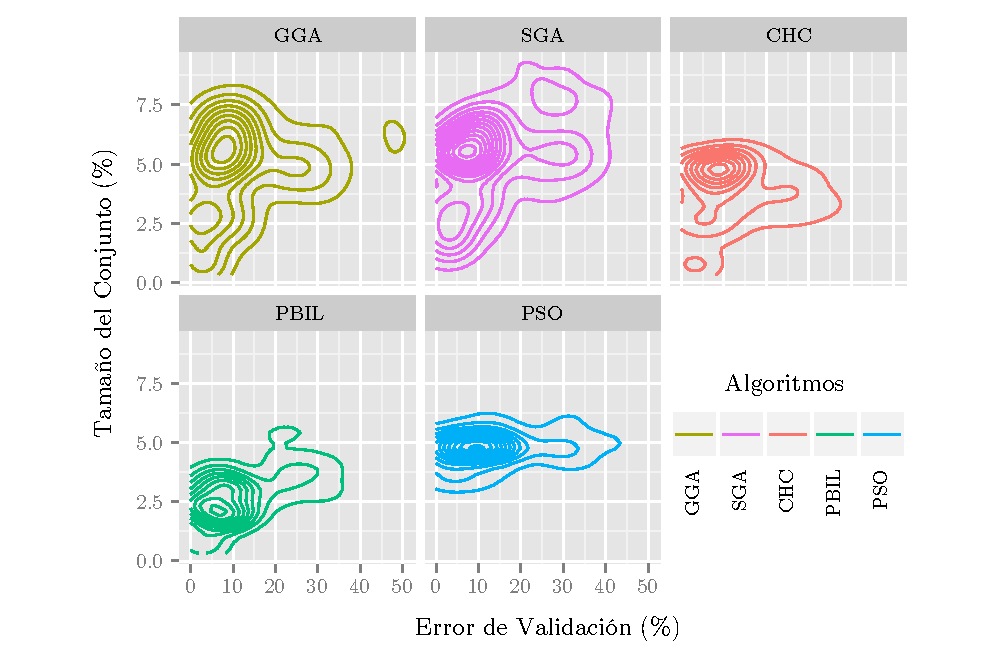
\includegraphics[width=\textwidth]{alg-density.pdf}
\caption[Distribución de los resultados de cada metaheurística]{Distribución de los resultados de cada metaheurística,\\en función del error de validación y el tamaño de las soluciones.}
\label{fig-alg-density}
\end{figure}

Esta gráfica confirma las conclusiones obtenidas a través de los datos presentados: PBIL muestra los mejores resultados en función de los objetivos del problema de SI. En comparación con las demás metaheurísticas, PBIL exhibe un comportamiento más estable, \emph{i.e.} la mayoria de sus soluciones presentan bajos porcentajes de error y tamaño. Al comparar estos datos con los de GGA, la gráfica de densidad muestra que los resultados de PBIL están mucho más concentrados en un área particular del plano, mientras que GGA presenta mayor variabilidad.

Para poder determinar con seguridad las posibles diferencias entre PBIL y el resto de las metaheurísticas, es necesario aplicar una prueba estadística. Se usa una prueba de rangos con signo de \emph{Wilcoxon} \cite{wilcoxon1945individual} (de cola inferior), con un nivel de significancia del $1\%$, para determinar si la mediana de la resultados de PBIL es menor que la de los resultados de las demás metaheurísticas en términos de error de validación o tamaño. A continuación se establecen las hipotesis de la prueba para este caso particular:

\begin{tabular}{l l}
$H_0$ & Los resultados de PBIL son mayores o iguales que los del algoritmo en cuestión.\\
$H_1$ & Los resultados de PBIL son menores que los del algoritmo en cuestión.\\
\end{tabular}

En función de estas hipótesis, en la tabla \ref{wilcox-res-pbil} se presenta el estadístico $W$ y el $p$-valor que permitirán rechazar o no la hipótesis nula $H_0$.

\begin{table}[h!]
\centering
\begin{tabular}{l c c c c}
\hline
\multirow{2}{*}{\textsc{Algoritmo}}
	& \multicolumn{2}{c}{\textsc{Error de Validación}}
	& \multicolumn{2}{c}{\textsc{Tamaño}} \\\cline{2-5}
 & $W$ & $p$-valor & $W$ & $p$-valor \\
\hline
\hline
GGA & 46 & $3.574 \times 10^{-1}$ &  1 & $1.221 \times 10^{-4}$ \\
SGA & 27 & $5.945 \times 10^{-2}$ &  0 & $6.104 \times 10^{-5}$ \\
CHC &  6 & $8.545 \times 10^{-4}$ & 14 & $6.714 \times 10^{-3}$ \\
PSO &  6 & $8.545 \times 10^{-4}$ &  0 & $6.104 \times 10^{-5}$ \\
\hline
\end{tabular}
\caption[Pruebas de \emph{Wilcoxon} comparando PBIL]{Estadístico $W$ y $p$-valor de pruebas de rangos con signo de \emph{Wilcoxon} para determinar si PBIL es mejor que el resto de las metaheurísticas, en función del error de validación y el tamaño de las soluciones encontradas.}
\label{wilcox-res-pbil}
\end{table}

Estos resultados permiten afirmar con un nivel de significancia del $1\%$, que PBIL exhibe mejores resultados que
\begin{inparaenum}[\itshape a\upshape)]
\item todas las metaheurísticas en términos de la reducción de los datos, y que
\item CHC y PSO en función al error de validación.
\end{inparaenum}
En resumidas cuentas, para encontrar soluciones al problema de SI, PBIL resulta la mejor opción en función de los objetivos del problema.

Sin embargo, debido a que el objetivo de estos algoritmos es que se apliquen sobre conjuntos de datos de tamaños grandes (mucho mayores a los conjuntos de datos evaluados en este estudio), la métrica del tiempo de ejecución es particularmente importante para evaluar las capacidades de las metaheurísticas para escalar a conjuntos mayores.

En este sentido, en la figura \ref{fig-tiempo} se grafica el aumento en tiempo de ejecución de las metaheurísticas en función del número de instancias de los 14 conjuntos de datos evaluados. Mientras que GGA, SGA, PBIL y PSO exhiben un aumento sustancial en el tiempo de ejecución, resulta evidente que CHC se ve menos afectado por el número de instancias que el resto de las metaheurísticas. Es destacable que CHC logre, en un tiempo significativamente menor, resultados competitivos en función del tamaño de las soluciones encontradas y manteniendo un error de validación aceptable. Esto hace de CHC el candidato perfecto para ser aplicado bajo conjuntos de datos con gran número de instancias.

\begin{figure}[h!]
\centering
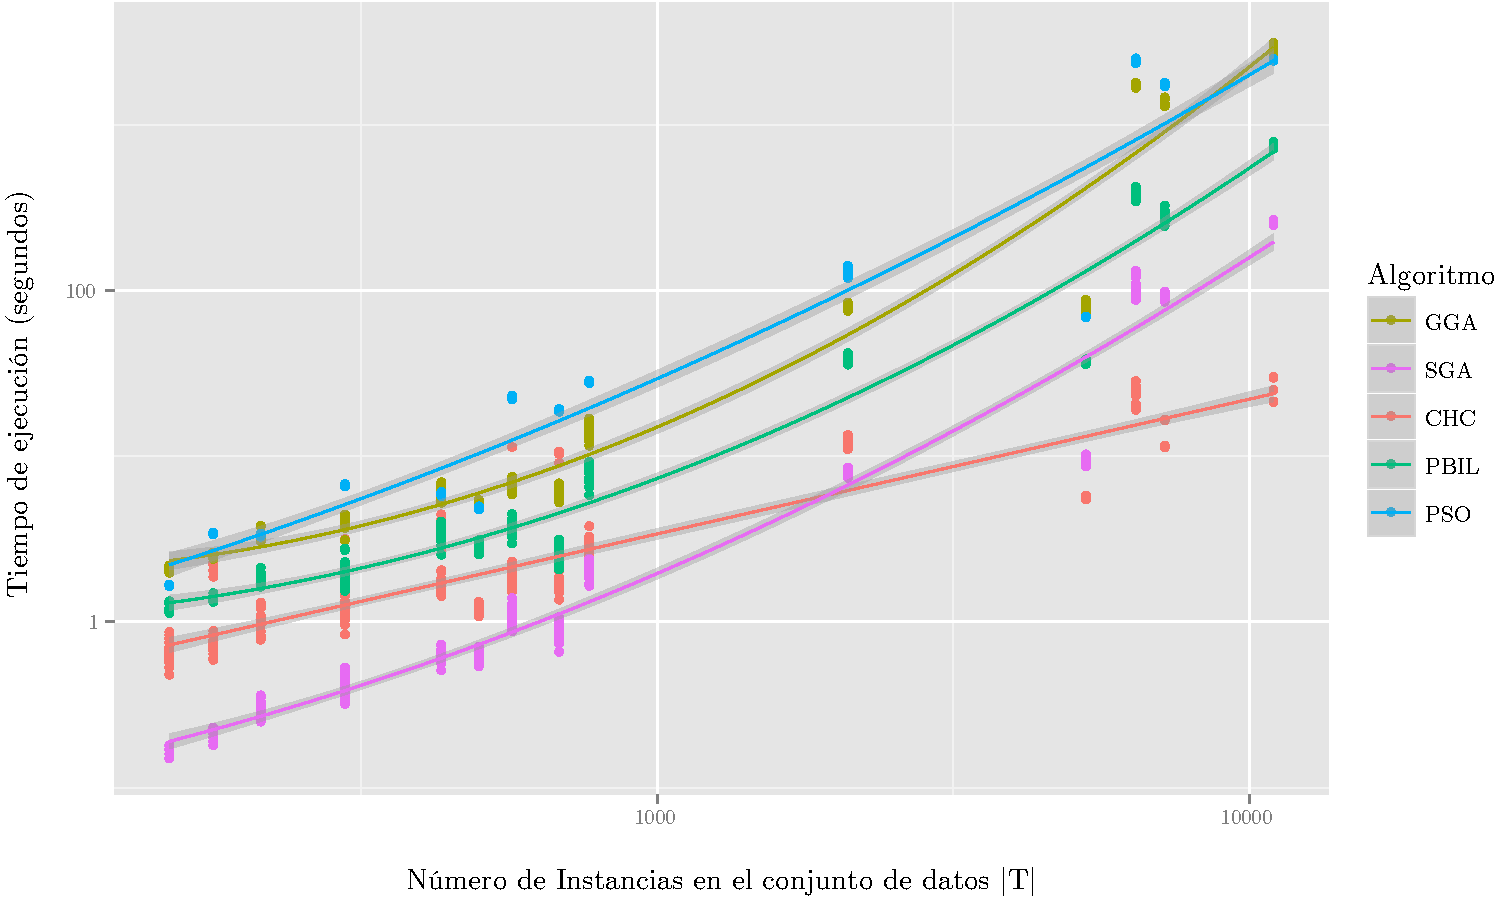
\includegraphics[width=0.9\textwidth]{tiempo.pdf}
\caption[Tiempo de ejecución de cada metaheurística]{Tiempo de ejecución reportado por cada metaheurística, usando el tiempo promedio en cada conjunto de datos, ordenándolos en función del número de instancias en cada conjunto de datos. Se usa escala logarítmica en ambos ejes.}
\label{fig-tiempo}
\end{figure}


% +--------------+
% | CONCLUSIONES |
% +--------------+
\chapter*{Conclusiones y Recomendaciones}
\label{conclusiones}
\lhead{\emph{Conclusiones y Recomendaciones}}
\addcontentsline{toc}{chapter}{Conclusiones y Recomendaciones}

En el presente trabajo fueron implementadas 5 metaheurísticas bio-inspiradas (\emph{i.e.} GGA, SGA, CHC, PBIL y PSO) para encontrar soluciones al problema de Selección de Instancias. Para esto, se propusieron (en función de los objetivos del problema) una serie de modificaciones a las estrategias de generación de soluciones iniciales al problema, usadas por las metaheurísticas como punto inicial del proceso de búsqueda. Adicionalmente, se realizó un estudio comparativo entre las metaheurísticas implementadas.%, para determinar aquellas metaheurísticas con mayor capacidad para encontrar soluciones al problema.

Los aportes de este trabajo se centran en las modificaciones realizadas sobre la generación de soluciones iniciales. En primer lugar, se propuso disminuir la probabilidad de aparición de bits $\delta$ (normalmente fijada en $50\%$), con la finalidad de reducir la cardinalidad de las soluciones iniciales generadas. Al usar una probabilidad igual al $5\%$, se lograron los objetivos planteados en términos del tamaño de las soluciones, además de una disminución considerable en el tiempo de ejecución; todo esto sin afectar de manera significativa en el error de clasificación.

Adicionalmente, se propuso modificar la probabilidad de aparición de cada bit de forma individual, aumentanto la probabilidad de aparición de las instancias seleccionadas por algoritmos heurísticos al problema de SI. En este sentido, se evaluó el impacto de usar probabilidades en función de las soluciones generadas por CNN, NEHS, Closest NE y Farthest NE, en contraste con el uso de una probabilidad constante. Contario a lo esperado, esta estrategia no resultó particularmente beneficiosa; únicamente la probabilidad en base a la selección de NEHS logró resultados comparables (y en algunos casos mejores) con el uso de una probabilidad constante.

Una vez determinadas las estrategias a seguir para la generación de solucines, se procedió a realizar un estudio comparativo entre las metaheurísticas implementadas, con la finalidad de determinar aquellas metaheurísticas que se comportan consistentemente mejor que las demás. De los resultados obtenidos, se concluye que PBIL encuentra las mejores soluciones en función de los objetivos del problema de SI. Sin embargo, el tiempo de ejecución de PBIL se ve muy afectado por el número de instancias en los conjuntos de datos. En este sentido, los resultados reportados por CHC lo convierten en una opción a considerar al momento de buscar soluciones al problema de SI sobre conjuntos de datos de tamaños mayores a los evaluados en este estudio.

En función del trabajo realizado, existen algunos aspectos relevantes a tomar en cuenta en futuros estudios sobre el problema de SI. A continuación se presentan algunas direcciones para expandir el presente estudio:

\begin{itemize}
\item Emplear una evaluación estratificada (como la descrita por \cite{cano2003using}) para encontrar soluciones a conjuntos de tamaño mayor que los usados en el presente trabajo.
\item Analizar el impacto de generar soluciones iniciales mediante algoritmos heurísticos, en el proceso de búsqueda llevado a cabo por metaheurísticas de trayectoria.
\item Evaluar adaptaciones alternativas de PSO para encontrar soluciones con representación binaria, con el objetivo de reducir el impacto que tiene el tamaño de los conjuntos de datos sobre su tiempo de ejecución.
\item Profundizar el estudio de NEHS (y algoritmos básados en ideas similares), para determinar su capacidad para conseguir soluciones al problema de SI.
\end{itemize}


% +--------------+
% | BIBLIOGRAFIA |
% +--------------+
\label{Bibliography}
\bibliography{bibliografia}
\lhead{\emph{Bibliografía}}
\bibliographystyle{alpha}
\addtocontents{toc}{\vspace{2em}}

% +-----------+
% | APENDICES |
% +-----------+
%\appendix
%\chapter{Entonación de las metaheurísticas}
\label{apendiceA}
\lhead{Apéndice A. \emph{Entonación de las metaheurísticas}}

En este apéndice se describe la metodología seguida durante el proceso de entonación de las metaheurísticas descritas en el Capítulo \ref{capitulo2}. Por cada metaheurística se describen los valores evaluados para cada parámetro y se presentan los resultados obtenidos de la experimentación. Estos experimentos fueron realizados usando \emph{Banana} como conjunto de datos de entonación, realizando 30 ejecuciones por cada configuración (3 repeticiones por cada \emph{fold}).

Cade destacar, que para las metaheurísticas GGA, SGA y PBIL se fijó el valor de la probabilidad de mutación en 0.001. Este debe ser un valor pequeño para no convertir el proceso de búsqueda en uno aleatorio, y el valor seleccionado ha sido usado en otros estudios \cite{cano2003using}. El resto de parámetros de cada metaheurística fue entonado, y sus resultados se presentan a continuación.

\section{Entonación de GGA}

Los parámetros de los que depende GGA son: el número de iteraciones, el tamaño de la población y la probabilidad de cruce (la prob. de mutación ya está fijada). En la tabla \ref{table-ap-gga} se presentan los diferentes valores evaluados para cada metaheurística. En este sentido, se realizó un estudio factorial para determinar el impacto de cada valor por separado y la interacción entre valores de diferentes parámetros.

\begin{table}[h!]
\centering
\begin{tabular}{l c}
\hline
\textsc{Parámetro} & \textsc{Valores Evaluados} \\
\hline
\hline
Iteraciones & 100\ \ \textbf{1000}\ \ 10000 \\
Población   & 10\ \ 20\ \ 30\ \ 40\ \ \textbf{50} \\
Prob. de Cruce & 0.5\ \ 0.6\ \ 0.75\ \ \textbf{0.9}\ \ 1.0\\
\hline
\end{tabular}
\caption[Valores evaluados para los parámetros de GGA]{Valores evaluados para los parámetros de GGA.\\En negrita los valores fijados por cada parámetro.}
\label{table-ap-gga}
\end{table}

En la figura \ref{fig-ap-gga} se presentan los resultados obtenidos de este estudio. Resulta evidente la existencia de un impacto inversamente proporcional entre el tamaño de población y el error de validación. Con una población de tamaño 50, GGA logra los mejores resultados.
Adicionalmente, los mejores resultados se obtienen mediante el uso de una probabilidad de cruce igual a 1.0 o 0.9, favoreciendo ligeramente a la selección de una probabilidad igual a 0.9.
Sin embargo, los resultados en función del número de iteraciones no son concluyentes, puesto que los resultados exhiben un comportamiento errático. Se selecciona un número de iteraciones igual a 1000.

\begin{figure}[h!]
\centering
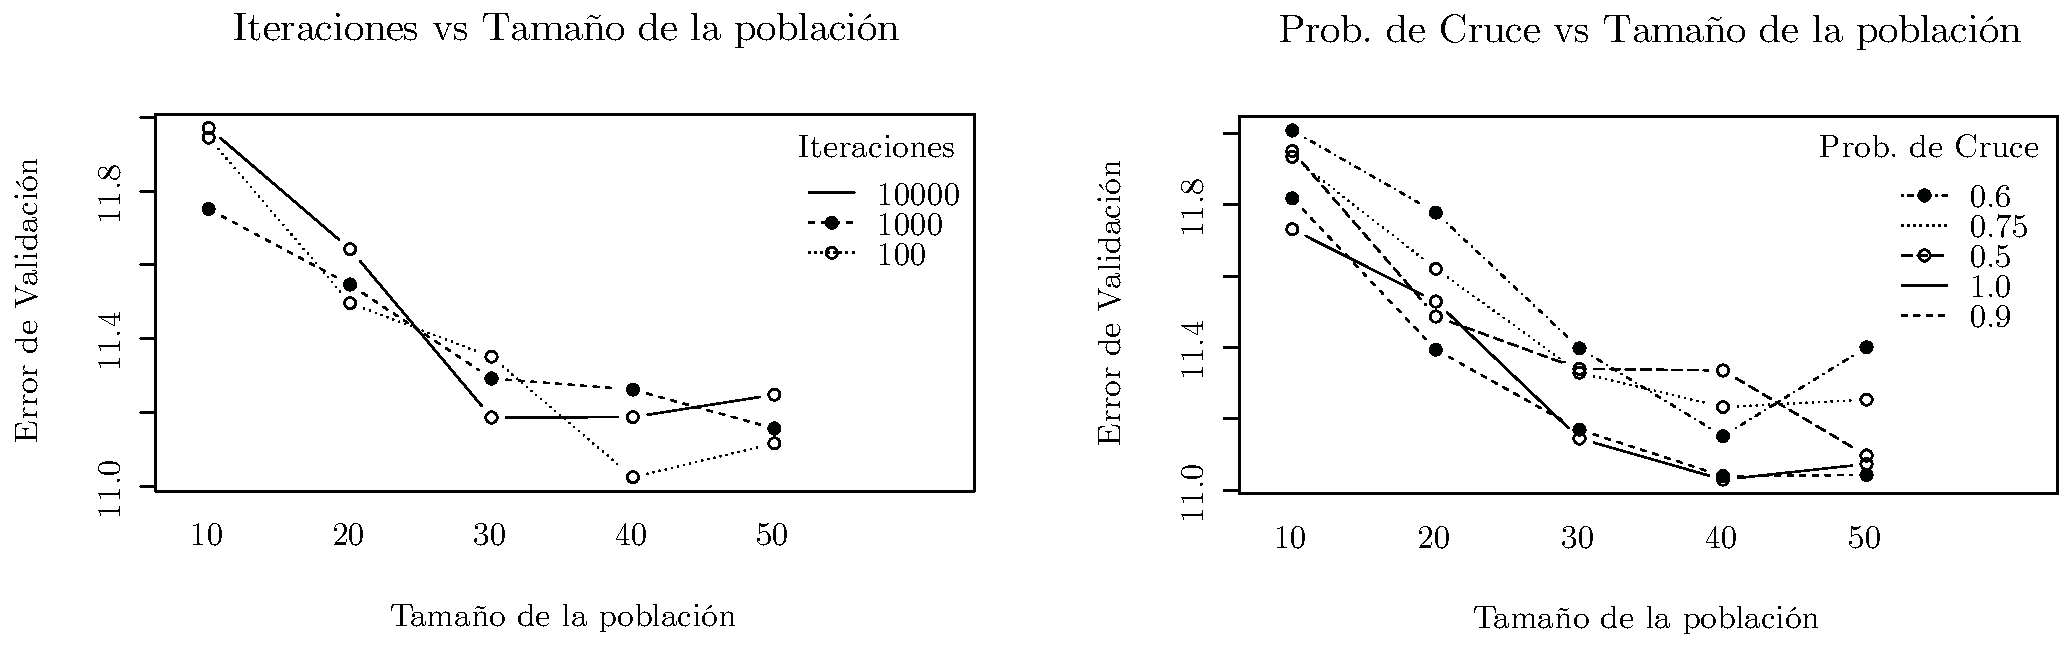
\includegraphics[width=\textwidth]{apendice-gga.pdf}
\caption{Resultados de entonación de GGA}
\label{fig-ap-gga}
\end{figure}

\section{Entonación de SGA}

SGA depende de los mismos parámetros que GGA. Por esta razón, se evalúan los mismos valores, descritos en la tabla \ref{table-ap-sga}. A partir de estos niveles de evaluación, se realiza un estudio factorial entre todos los parámetros.

\begin{table}[h!]
\centering
\begin{tabular}{l c}
\hline
\textsc{Parámetro} & \textsc{Valores Evaluados} \\
\hline
\hline
Iteraciones & 100\ \ \textbf{1000}\ \ 10000 \\
Población   & 10\ \ 20\ \ \textbf{30}\ \ 40\ \ 50 \\
Prob. de Cruce & 0.5\ \ 0.6\ \ 0.75\ \ 0.9\ \ \textbf{1.0}\\
\hline
\end{tabular}
\caption[Valores evaluados para los parámetros de SGA]{Valores evaluados para los parámetros de SGA.\\En negrita los valores fijados por cada parámetro.}
\label{table-ap-sga}
\end{table}

Al comparar los resultados presentados en la figura \ref{fig-ap-sga}, resulta evidente el efecto positivo de aumentar el número de iteraciones en SGA. Sin embargo, a pesar de que los resultados favorecen ampliamente el uso de 10000 iteraciones, esto implica un aumento de un orden de magnitud en el tiempo de ejecución de la metaheurística. Esto lleva a la selección de un número de iteraciones intermedio (1000) que genere soluciones aceptables sin incurrir en altos costos de cómputo.

Adicionalmente, los resultados presentados en función del tamaño de la población usada, llevan a concluir que este parámetro no influye significativamente en el proceso de búsqueda de SGA. Se selecciona el nivel medio, igual a 30 individuos.

Por último, el efecto la probabilidad de cruce es poco claro. Se decide seleccionar una probabilidad de cruce igual a 1.0 para asegurar la generación de nuevos individuos en cada iteración.

\begin{figure}[h!]
\centering
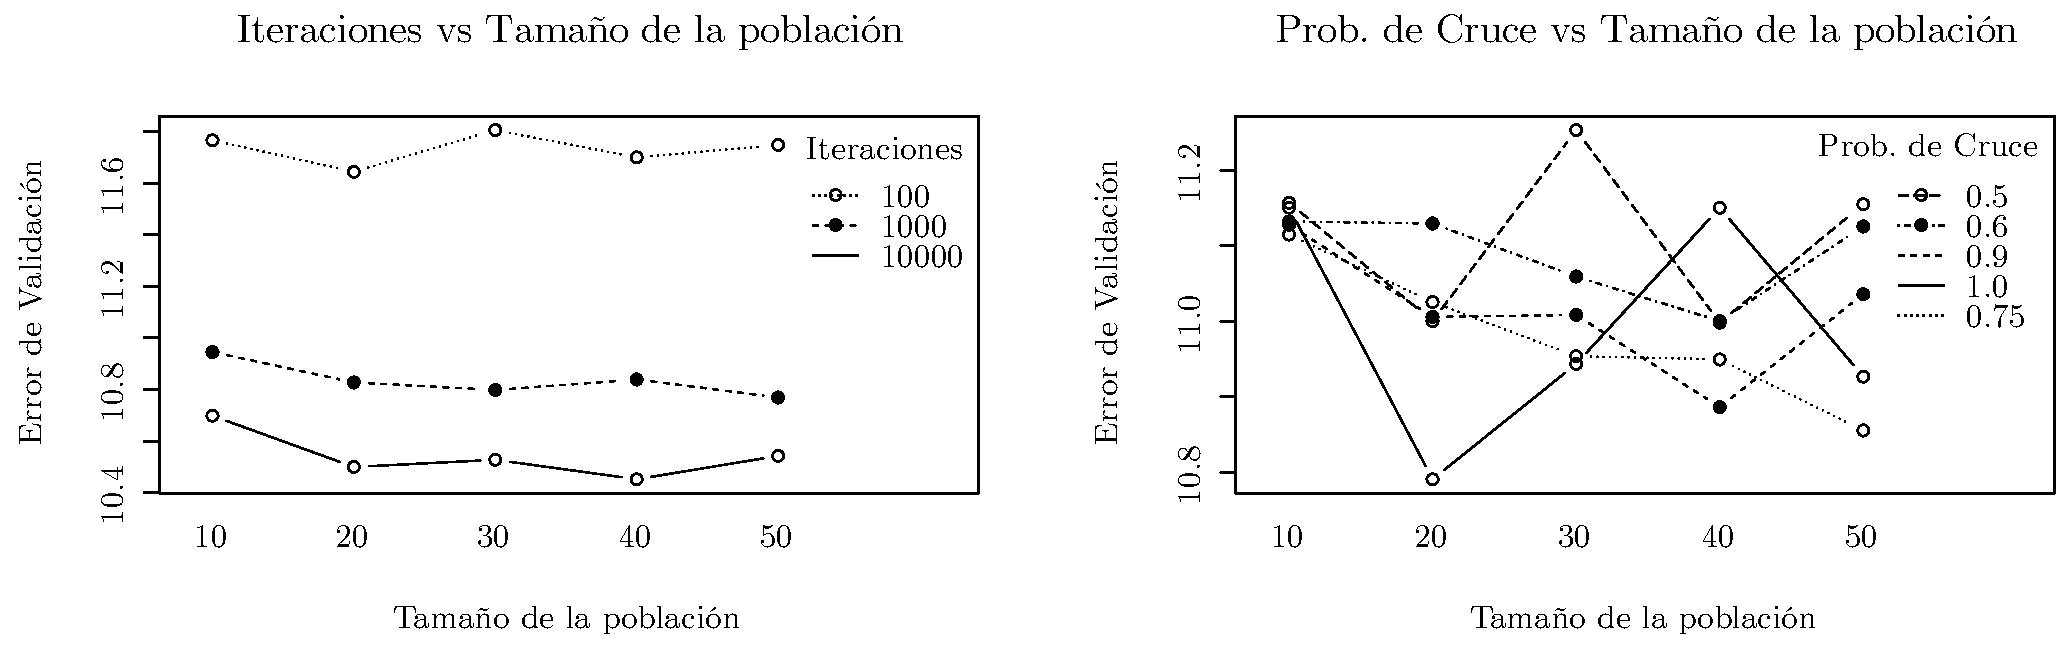
\includegraphics[width=\textwidth]{apendice-sga.pdf}
\caption{Resultados de entonación de SGA}
\label{fig-ap-sga}
\end{figure}

\section{Entonación de CHC}

CHC es la metaheurística con menos parámetros que entonar. Tan solo depende del número de iteraciones y el tamaño de la población. Los valores evaluados son descritos en la tabla \ref{table-ap-chc}.

\begin{table}[h!]
\centering
\begin{tabular}{l c}
\hline
\textsc{Parámetro} & \textsc{Valores Evaluados} \\
\hline
\hline
Iteraciones & 100\ \ \textbf{1000}\ \ 10000 \\
Población   & 10\ \ 20\ \ \textbf{30}\ \ 40\ \ 50 \\
\hline
\end{tabular}
\caption[Valores evaluados para los parámetros de CHC]{Valores evaluados para los parámetros de CHC.\\En negrita los valores fijados por cada parámetro.}
\label{table-ap-chc}
\end{table}

Los resultados presentados en la figura \ref{fig-ap-chc} son claros y las conclusiones evidentes. El comportamiento de la metaheurística luego de 1000 o 10000 iteraciones es muy similar, y es poco dependiente del tamaño de la población. Se escoge un tamaño de población medio (igual a 30) y un número de iteraciones igual 1000 para reducir el tiempo de ejecución.

\begin{figure}[h!]
\centering
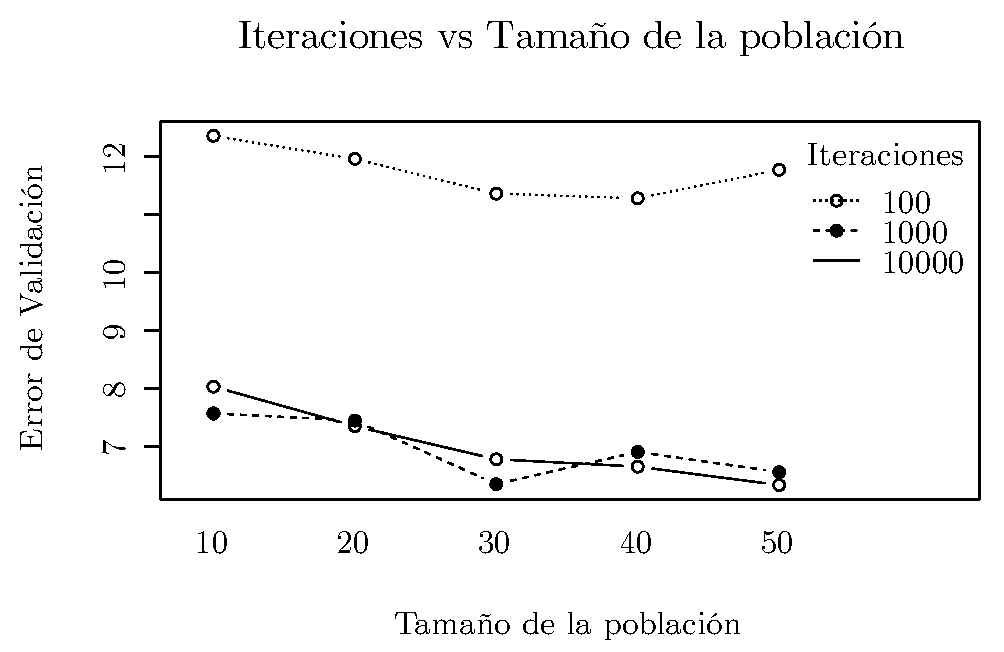
\includegraphics[width=0.5\textwidth]{apendice-chc.pdf}
\caption{Resultados de entonación de CHC}
\label{fig-ap-chc}
\end{figure}

\section{Entonación de PBIL}

La entonación de PBIL resulta más complicada, debido a que depende de un mayor número de parámetros. En la tabla \ref{table-ap-pbil} se describen los valores evaluados para cada parámetro. Se excluye de este estudio el valor de \emph{Mutation Shift}, que se mantiene en un valor bajo (igual a 0.01). Con los niveles descritos por cada parámetro, se realiza un estudio factorial.

\begin{table}[h!]
\centering
\begin{tabular}{l c}
\hline
\textsc{Parámetro} & \textsc{Valores Evaluados} \\
\hline
\hline
Iteraciones & 100\ \ \textbf{1000}\ \ 10000 \\
Población   & 10\ \ 20\ \ 30\ \ \textbf{40}\ \ 50 \\
Learning Rate & \textbf{0.1}\ \ 0.05\ \ 0.01 \\
Negative Learning Rate & 0.075\ \ 0.05\ \ \textbf{0.01} \\
\hline
\end{tabular}
\caption[Valores evaluados para los parámetros de PBIL]{Valores evaluados para los parámetros de PBIL.\\En negrita los valores fijados por cada parámetro.}
\label{table-ap-pbil}
\end{table}

De los resultados obtenidos (ver figura \ref{fig-ap-pbil}), se derivan las siguientes conclusiones:
\begin{itemize}
\item El tamaño de la población y el número de iteraciones influyen significativamente en la disminución del error de validación. Aplicando 1000 iteraciones, los mejores resultados son obtenidos con poblaciones de tamaño 40.
\item Existe una relación importante entre los valores de \emph{Learning Rate} y el \emph{Negative Learning Rate}. La combinación de 0.1 y 0.01 respectivamente, prueba ser la mejor alternativa. Esta conclusión se ratifica al evaluar la interacción entre ambos parámetros y el número de iteraciones.
\end{itemize}

\begin{figure}[h!]
\centering
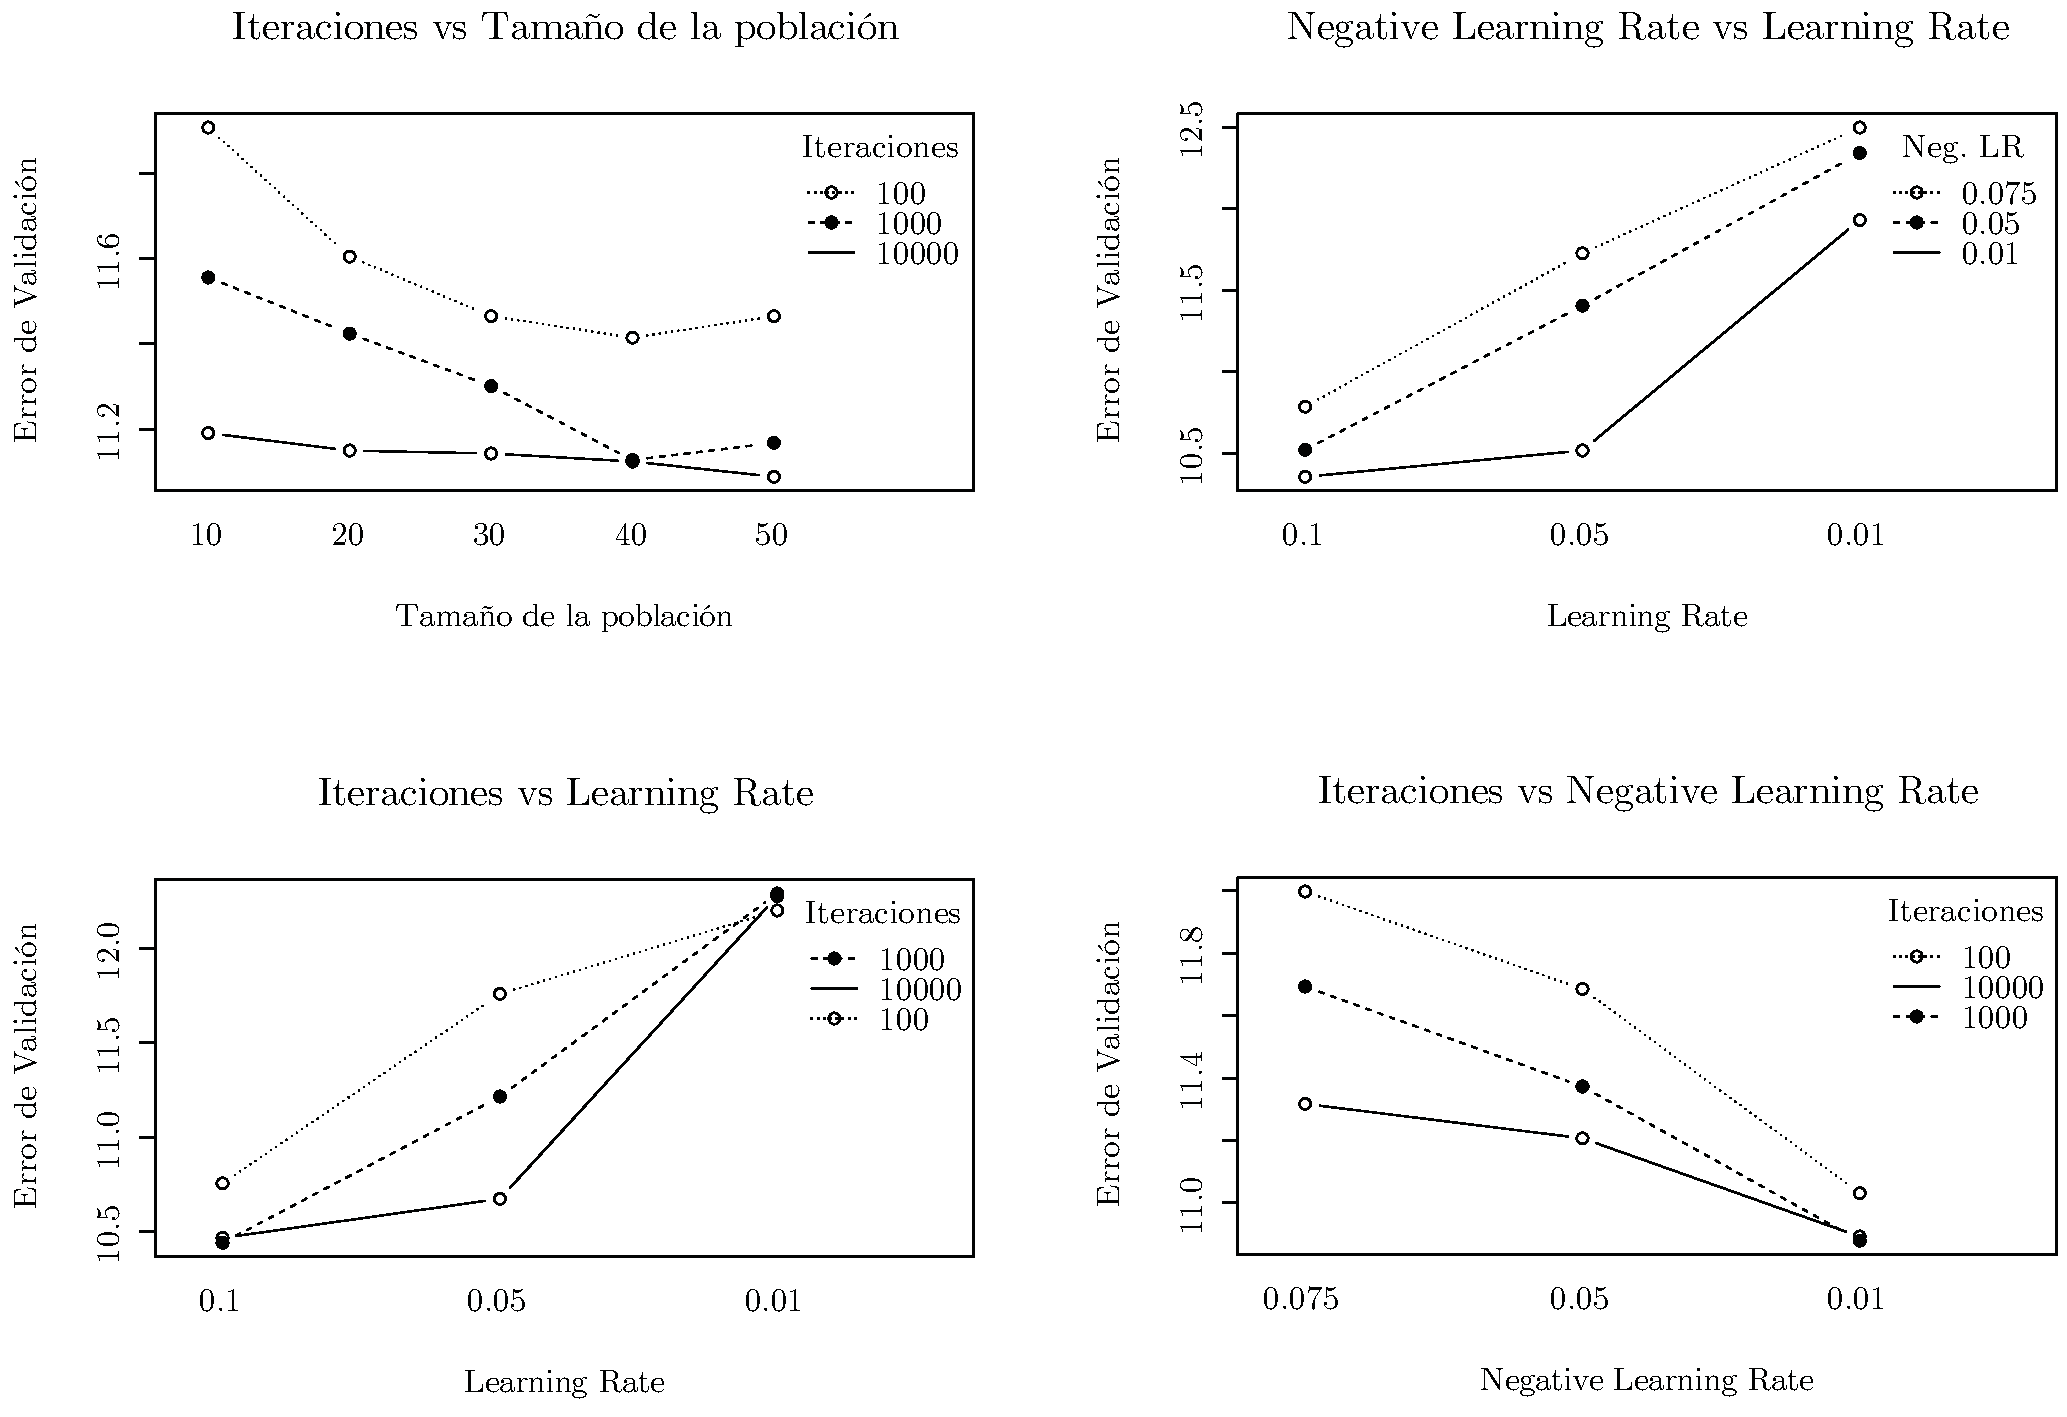
\includegraphics[width=\textwidth]{apendice-pbil.pdf}
\caption{Resultados de entonación de PBIL}
\label{fig-ap-pbil}
\end{figure}

\section{Entonación de PSO}

En la tabla \ref{table-ap-pso} se describen los valores utilizados para evaluar el impacto de algunos de los parámetros de los que depende PSO. El resto de los parámetros fueron fijados con la finalidad de limitar el impacto en tiempo sobre el algoritmo. PSO se vio especialmente afectado en tiempo de ejecución por el número de iteraciones, por lo que se decidió fijar este parámetro en 1000 al igual que el resto de las metaheurísticas. Adicionalmente, debido a que el número de soluciones generadas por PSO en cada iteración es igual al número de partículas por el tamaño de la población, se fijó este último parámetro en 5 individuos para evitar un aumento considerable en el tiempo de ejecución y evaluar el impacto del aumento de las partículas. Por último, las constantes $c1$ y $c2$ se fijan en función de la velocidad máxima (\emph{i.e.} $\frac{\texttt{vmax}}{2}$) pues no tiene sentido usar valores más altos dado que el vector de velocidad está acotado por $\texttt{vmax}$.

\begin{table}[h!]
\centering
\begin{tabular}{l c}
\hline
\textsc{Parámetro} & \textsc{Valores Evaluados} \\
\hline
\hline
Partículas  & \textbf{5}\ \ 10\ \ 15 \\
Inercia ($w$) & \textbf{0.9}\ \ 0.6\ \ 0.3 \\
Velocidad Máxima (\texttt{vmax}) & 0.5\ \ \textbf{0.2}\ \ 0.05 \\
\hline
\end{tabular}
\caption[Valores evaluados para los parámetros de PSO]{Valores evaluados para los parámetros de PSO.\\En negrita los valores fijados por cada parámetro.}
\label{table-ap-pso}
\end{table}

Para los valores de Inercia y Velocidad Máxima, se realizó un estudio factorial, y los resultados son presentados en la figura \ref{fig-ap-pso}. Resulta clara la interacción entre diferentes valores de estos parámetros, donde la combinación de una inercia igual a 0.9 y una velocidad máxima de 0.2 logran los mejores resultados.

El número de partículas fue evaluado de forma independiente. Los resultados obtenidos muestran que no existen diferencias en el uso de diferentes números de partículas. Este parámetro se fija en 5 partículas con la finalidad de disminuir el tiempo de ejecución del algoritmo.

\begin{figure}[h!]
\centering
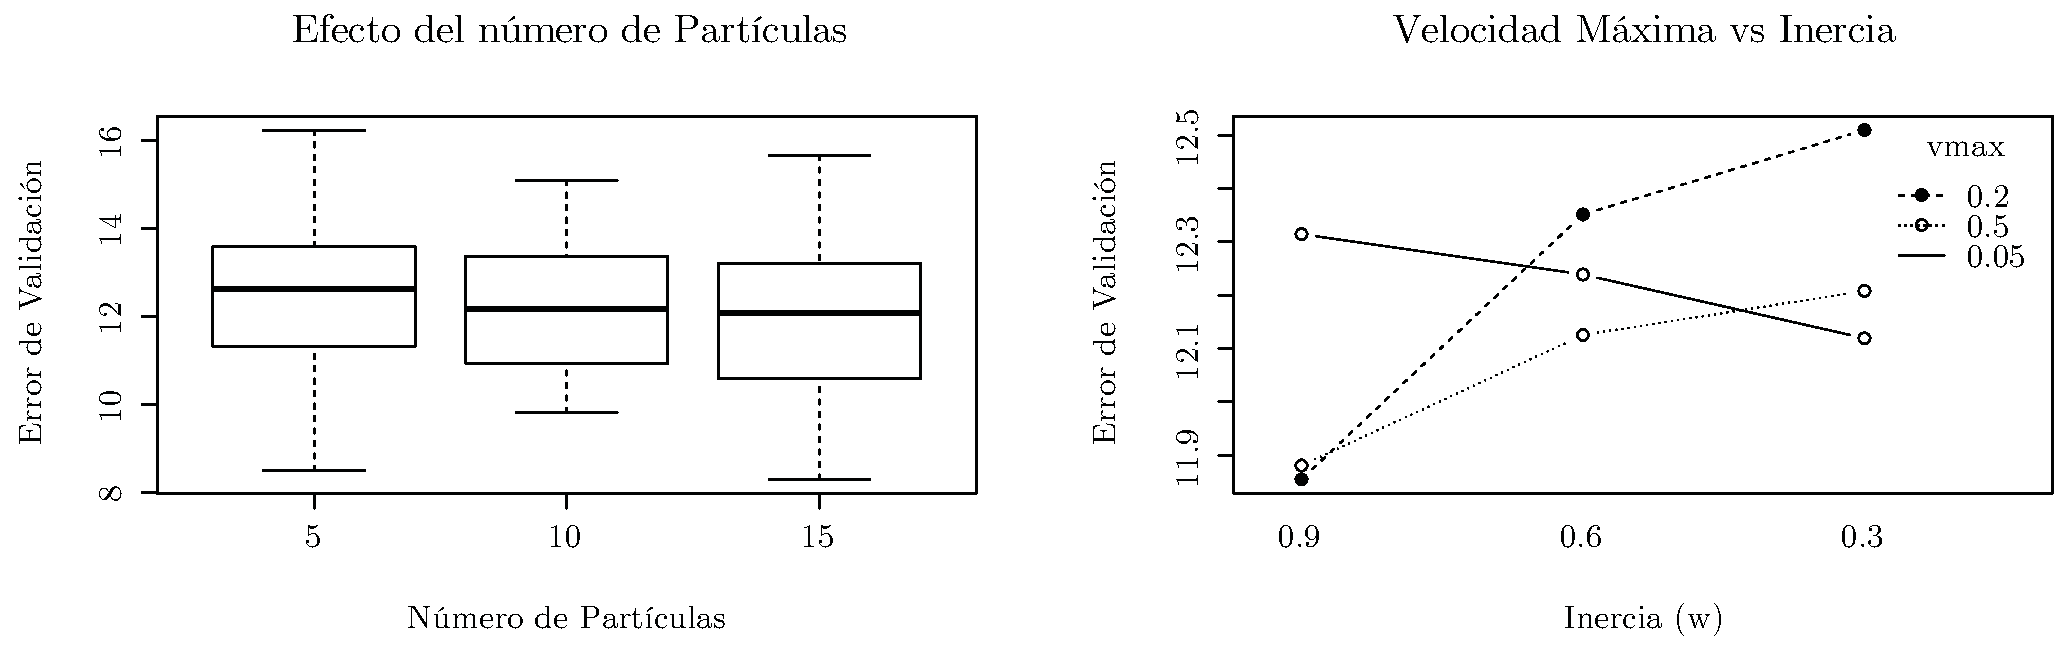
\includegraphics[width=\textwidth]{apendice-pso.pdf}
\caption{Resultados de entonación de PSO}
\label{fig-ap-pso}
\end{figure}

%\chapter{@nombreApendice}
\label{apendiceB}
\lhead{Apéndice B. \emph{@nombreApendice}}

\Blindtext

%\addtocontents{toc}{\vspace{2em}}

\backmatter

\end{document}
